%% GigaScience Research article. Generated by scripts/giga_build.py from
%% submission/dkd-manuscript.tex; edit that file and rebuild, do not edit this one.
\documentclass[11pt,a4paper]{article}
\PassOptionsToPackage{hyphens}{url}
\usepackage[a4paper,margin=25mm]{geometry}
\usepackage[T1]{fontenc}
\usepackage{lmodern}
\usepackage{cmap}
\usepackage{graphicx,booktabs,array,multirow,amsmath,amssymb,amsfonts,textcomp,url,xcolor}
\usepackage{setspace}
\usepackage[numbers,square,sort&compress]{natbib}
\usepackage[hidelinks]{hyperref}
\graphicspath{{figures/}}
\providecommand{\bibcommenthead}{}
\providecommand{\botrule}{\bottomrule}
\providecommand{\bmhead}[1]{\subsection*{#1}}
\renewcommand{\footnotetext}[1]{\par\smallskip{\footnotesize #1}}
\setlength{\parskip}{4pt}
\emergencystretch=3em
\renewcommand{\topfraction}{0.9}\renewcommand{\bottomfraction}{0.7}
\renewcommand{\textfraction}{0.08}\renewcommand{\floatpagefraction}{0.75}
\raggedbottom
\begin{document}
\doublespacing
\begin{center}
{\Large \bfseries Auditing cross-cohort feature-selection benchmarks: cohort composition and tissue-context-dependent confounding across kidney, liver and colon transcriptomes}\\[10pt]
Dohun Kim\textsuperscript{1}\textsuperscript{*}, Minho Bae\textsuperscript{1}, Jinho Park\textsuperscript{1}, Hayoung Lee\textsuperscript{1}, Hyeokjin Lim\textsuperscript{1} and Seonghee Lee\textsuperscript{1}\\[6pt]
{\small \textsuperscript{1}Autonomous Intelligence DX Research Section, Electronics and Telecommunications Research Institute, Daejeon, Republic of Korea}\\
{\small \textsuperscript{*}Corresponding author: Dohun Kim, \href{mailto:dohun@etri.re.kr}{dohun@etri.re.kr}}\\[2pt]
{\small Author e-mail addresses: Dohun Kim, dohun@etri.re.kr; Minho Bae, minkkang@etri.re.kr; Jinho Park, jinho.park@etri.re.kr; Hayoung Lee, underzero11@etri.re.kr; Hyeokjin Lim, hyeokjin.lim@etri.re.kr; Seonghee Lee, slee0003@etri.re.kr}
\end{center}
\bigskip
\section*{Abstract}
\textbf{Background:} Cross-cohort feature selection is widely used to derive reproducible transcriptomic biomarker signatures from public cohorts. This assumes that reproducibility reflects disease biology and that the benchmark measures the methods rather than the cohorts. We tested both in diabetic kidney disease, then in liver and colon against predictions fixed in advance.

\textbf{Results:} Over all 26 subsets of five discovery cohorts, reproducibility verdicts were unstable: a stability-selection strategy won cross-fold agreement in 9 of 10 three-cohort subsets yet lost on all five, while its external AUROC advantage stayed positive. The most reproducible signal tracked procurement, not disease: an immediate-early gene module separated biopsy from surgical tissue in 8 of 9 kidney datasets, and a biopsy control retained only 14--56\% of the naive signal across seven diagnoses. Residualising on a handling score cut procurement-driven genes from 27\% to 5\% with no AUROC loss detected on a wide interval; batch correction by cohort was inert. In liver and colon the module was lower in biopsy cases than surgical controls in 9 of 10 such cohorts, verdict instability recurred in liver but not colon, and the module rose with inflammation, failing one prediction.

\textbf{Conclusions:} Without a cohort-composition sensitivity analysis, a cross-cohort reproducibility comparison describes the cohorts rather than the methods, and should be reported separately from predictive performance. A shared pre-analytical confounder becomes reproducible wherever the design is shared; removing it rewrites the candidate list, 14 of 30 genes surviving. We release the harmonised cohorts, the schema-enforced audit database, the candidate-evidence ledger and the regenerating pipeline.

\noindent\textbf{Keywords:} feature selection; benchmarking; reproducibility; batch effects; pre-analytical variables; diabetic kidney disease; transcriptomics

\section{Background}\label{sec:background}
%%=============================================================%%

Transcriptomic biomarker discovery in chronic kidney disease has converged on a common recipe:
assemble public case/control cohorts, select features that behave consistently across them, and
report the resulting signature with a classification performance figure. The appeal is that
consistency across independent cohorts should filter dataset-specific noise. A substantial
methods literature has developed around this idea, from multi-cohort meta-analysis
\cite{haynes2017} to stability-selection frameworks \cite{meinshausen2010}. The pitfalls of
deriving classifiers from high-dimensional expression data have been catalogued repeatedly
\cite{simon2003,whalen2022,diazuriarte2022}, as has the impact of batch and other technical
structure on such analyses \cite{leek2010}.

Two assumptions underlie the recipe. The first is that a feature reproducible across cohorts is
more likely to reflect disease biology. The second is that a benchmark comparing selection
methods on a set of public cohorts estimates something about the methods rather than about the
cohorts. This work tests both, in diabetic kidney disease (DKD), where the number of usable
public cohorts is small enough to enumerate exhaustively and large enough to resample, and
then asks whether what it finds there carries to two tissues whose cohorts are designed
differently.

Neither concern is new in the abstract. That the outcome of a method comparison depends on how
the comparison was set up (which datasets, which defaults, which analysis choices) has been
argued and demonstrated repeatedly in computational biology: in the case for neutral comparison
studies \cite{boulesteix2013}, in explicit illustrations of over-optimism
\cite{jelizarow2010,ullmann2023}, and in the benchmarking guidelines that grew out of them
\cite{weber2019,mangul2019}. A related bias is that method comparisons run by a method's own
authors tend to favour it \cite{norel2011}, and the same sensitivity has been described outside
biology as a benchmark lottery \cite{dehghani2021}. Separately, the instability of
high-dimensional feature selection under resampling is a standing result \cite{haury2011}.

A meta-analysis of 28 filter feature-selection studies found that the number of datasets,
baselines and new methods alone explained 33\% of the variance in reported win rates
\cite{ebiele2026}, and a recent framework grades which layers of differential-expression evidence
reproduce across fixed cohorts \cite{angelakis2026}; neither varies which cohorts enter the
comparison. What is missing is a quantification for cross-cohort omics biomarker discovery specifically,
where varying the cohort configuration is recommended practice but reporting the resulting
interval is not. We therefore treat the phenomenon as established and measure its magnitude in a
setting that has not accounted for it, alongside a concrete mechanism for one particular failure
and a benchmark of the corrections available for it.

This study makes five contributions. The first is a cohort-composition sensitivity analysis,
stated as a protocol rather than as a one-off check: the reproducibility comparison is reported
as an interval over every admissible subset of the discovery cohorts, so that a verdict which
depends on the configuration cannot be presented as a verdict about the methods. The second is a
control-definition sensitivity analysis, which replaces the non-biopsy control with a disease
control obtained through the same biopsy procedure. It separates a design effect from a disease
effect without collecting new samples, and it needs only cohorts that already exist. The third is
a benchmark of the corrections available for the confounder those two analyses expose, including
which corrections cannot work in this design and why. The fourth is the form of the output: an
auditable candidate-evidence ledger rather than a ranked gene list, recording for each candidate
the evidence lines it passed, the rank it takes under each control definition, and how far that
rank moves when the control group is substituted. The fifth is a test of whether the two
mechanisms are properties of cross-cohort benchmarking or of these kidney cohorts: three
predictions, written and hashed before any expression value was read, evaluated in liver, where
procurement is asymmetric in some cohorts and matched in others, and in colon, where it is
matched in all. One held, one held in one tissue, and one failed, and the failures narrow both
claims in ways the kidney data could not.

Figure~\ref{fig:overview} sets out the study workflow: audit the benchmark input, stress-test conclusions against cohort composition and control definition, then diagnose and correct the confounder before reporting an auditable candidate-evidence ledger. The cohort audit, the residual overlap it could not remove, and the discovery/validation split are described in Section~\ref{sec:cohorts}.

\begin{figure}[htbp]
% source: P0_overview
\centering
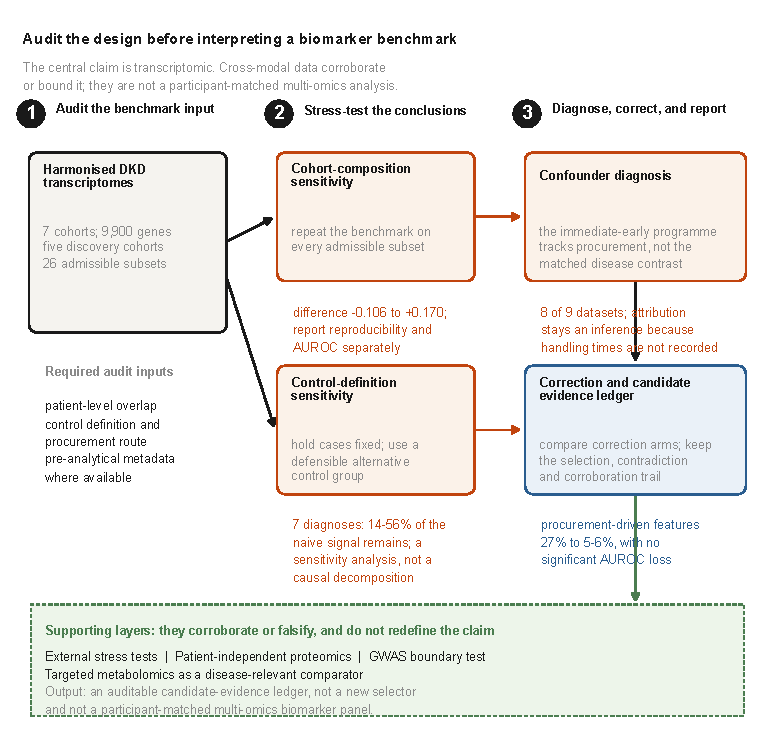
\includegraphics[width=\textwidth]{Fig1}
\caption{\textbf{Study workflow and scope.} The central analysis is a cross-cohort transcriptomic benchmark. It begins with patient-overlap and control-procurement audits, then applies two sensitivity analyses: cohort composition and control definition. These expose a procurement-associated immediate-early programme, whose attribution remains an inference because handling times were not recorded. Correction is evaluated by its removal of procurement-driven features and preservation of external AUROC; candidates are reported as an auditable evidence ledger rather than a ranked list alone. The lower band distinguishes supporting layers, which corroborate or falsify candidate claims, from participant-matched integrative multi-omics, which this study does not claim.}\label{fig:overview}
\smallskip\noindent{\footnotesize Alt text: Flow diagram of the study. Top row: audit the benchmark input for patient overlap and control procurement; then two sensitivity analyses, cohort composition and control definition; then diagnosis and correction of a procurement-associated immediate-early programme; then an auditable candidate-evidence ledger. A lower band separates supporting layers that corroborate or falsify candidates from participant-matched integrative multi-omics, which is marked as not claimed.}
\end{figure}


Both assumptions fail in ways that are measurable. Reproducibility is maximised by whatever is
most consistent across cohorts, and in this disease that turns out to be a shared pre-analytical
confounder rather than biology. Benchmark verdicts on reproducibility flip sign depending on
which cohorts are included. Neither failure is specific to a particular algorithm, and both are
invisible without the controls we describe.

%%=============================================================%%

\section{Data description}\label{sec:data}

\subsection{Cohort assembly and audit}\label{sec:cohorts}

Fifteen human DKD transcriptome series were retrieved from the Gene Expression Omnibus.
Sample-level metadata were parsed from series matrices and patient identifiers recovered from
sample titles, which revealed patient-level reuse invisible at the accession level. Three series
(GSE30122, GSE47183 and GSE99340) were excluded on this basis; Additional file~2 gives the evidence for each. Reusing them would have
inflated every cross-cohort statistic in this study, because the same patients would have
appeared in both the selection and the evaluation side of a leave-one-dataset-out split.

Residual overlap that could not be removed is disclosed rather than ignored (Table~\ref{tab:overlap}; Additional file~2 gives the full audit). It is larger than the DKD case counts alone suggest: GSE104948 and GSE104954 are the two compartments of one ERCB collection and share 55 subjects, of which 5 are DKD cases, 1 is a non-biopsy control and 49 are the non-diabetic kidney-disease biopsies that Section~\ref{sec:procurement} uses as the matched comparator. GSE30528 and GSE30529 share 9 subjects, 5 DKD cases and 4 controls. These are not duplicate cohorts; they are the same patients profiled in two compartments, which is what makes the paired analyses possible. The consequence is that the leave-one-dataset-out folds are not fully independent when both compartments are present, and we report it rather than treat the two as unrelated datasets. GSE104948 also enters the analysis twice: once as a discovery cohort and once as one of the two blocks of the DKD-versus-non-diabetic-CKD specificity gate (Section~\ref{sec:whichcorrections}). The gate is therefore not a fully independent validation of the candidates it filters. Independence was probed instead in the external GSE20602 cohort (Section~\ref{sec:external}), and a sensitivity analysis re-derives the candidates with GSE104948 removed from discovery (Section~\ref{sec:limitations}).

\begin{table}[h]
\caption{Subjects appearing in more than one retained series. These are the same patients profiled in two compartments, not duplicate cohorts.}\label{tab:overlap}
\begin{tabular}{@{}llrrrr@{}}
\toprule
Series A & Series B & Shared & DKD & Non-biopsy & Other \\
        &          & subjects & cases & controls & biopsy \\
\midrule
GSE104948 & GSE104954 & 55 & 5 & 1 & 49 \\
GSE30528 & GSE30529 & 9 & 5 & 4 & 0 \\
\botrule
\end{tabular}
\footnotetext{Other biopsy are the non-diabetic kidney-disease biopsies that Section~\ref{sec:procurement} uses as the procurement-matched comparator. They are counted here because the leave-one-dataset-out folds are not independent for those subjects either.}
\end{table}

Five cohorts entered the discovery rotation and two served as compartment validation
(Table~\ref{tab:cohorts}) \cite{woroniecka2011,pan2018,grayson2018,fan2019,jin2026}. One feature of that table carries the rest of this paper:
in every cohort the cases are kidney biopsies and the controls are not. None of the five
discovery contrasts uses a biopsy-matched control group; the biopsy comparators that do exist, in
ERCB and KPMP, are what the control-definition analyses below rely on. Additional cohorts
were used for specific tests: GSE175759 \cite{park2022}, GSE162830 \cite{eadon2021}, GSE142153 \cite{sur2021}, GSE1009 \cite{baelde2004}, GSE111154 \cite{sircar2018}, GSE20602 \cite{neusser2010}, the
Kidney Precision Medicine Project (KPMP) single-nucleus atlas \cite{elachkar2021,lake2023}, and GSE5406
(heart, external organ) \cite{hannenhalli2006}. KPMP does not enrol diabetic kidney disease as a category; the 27 single-nucleus donors enrolled with chronic kidney disease and a recorded history of diabetes are treated throughout as an operational DKD-proxy subset rather than a registry-defined diagnosis (Section~\ref{sec:limitations}). Three of the discovery cohorts were first described by Woroniecka et
al.\ \cite{woroniecka2011}.

\begin{table}[h]
\caption{Transcriptome cohorts used. Cases are kidney biopsies in every cohort; controls are not. This is the design feature Section~\ref{sec:procurement} tests.}\label{tab:cohorts}
\footnotesize
\setlength{\tabcolsep}{4pt}
\begin{tabular}{@{}llllrrl@{}}
\toprule
Cohort & Role & Compart. & Platform & Cases & Controls & Control tissue \\
\midrule
GSE104948 & discovery & glom. & GPL22945/GPL24120 & 12 & 26 & donor, nephrec. \\
GSE142025 & discovery & cortex & Illumina HiSeq4000 & 27 & 9 & nephrec. \\
GSE294519 & discovery & tubulo. & GPL24676 & 23 & 13 & nephrec. \\
GSE30528 & discovery & glom. & GPL571 & 9 & 13 & nephrec. \\
GSE96804 & discovery & glom. & GPL17586 & 41 & 20 & nephrec. \\
GSE104954 & compartment & tubulo. & GPL22945/GPL24120 & 17 & 26 & donor, nephrec. \\
GSE30529 & compartment & tubulo. & GPL571 & 10 & 12 & nephrec. \\
\botrule
\end{tabular}
\footnotetext{Compartments: glom., glomerulus; tubulo., tubulointerstitium; cortex, whole renal cortex. Control tissue: nephrec., tumour nephrectomy; donor, living kidney donor. All cohorts are expressed on the same frozen 9,900-gene Entrez space. Cohorts marked \emph{compartment} are the second compartment of donors already represented by an ERCB or Woroniecka series; they enter the procurement and comparator analyses but not the cohort-composition sweep, which requires independent cohorts.}
\end{table}

\subsection{Harmonisation}\label{sec:harmonisation}

Entrez Gene ID was used as the hub identifier because GSE104948 and GSE104954 use the Brainarray
ENTREZG custom CDF, so their probe identifiers already are Entrez IDs and the tightest cohort
suffers no mapping loss. Platform probes were mapped through GEO \texttt{.annot} files (GPL571,
GPL96, GPL8300, GPL6480), the GPL17586 platform table, and NCBI \texttt{gene\_info} for symbol-
and Ensembl-keyed matrices. Probes mapping to more than one gene were dropped. Where several
probes mapped to one gene the probe with the highest mean expression was retained (max-mean
collapse), a rule fixed before any analysis and applied identically everywhere, because changing
it invalidates every stability count computed on the resulting space.

The intersection over the four original discovery cohorts is 9,900 genes; adding the compartment
cohorts costs nothing since they share platforms. GSE294519 was mapped into this frozen space
rather than triggering re-derivation, and covers 98.5\% of it.

All cross-cohort operations use per-cohort gene-wise $z$-scores. Value scales differ
fundamentally between cohorts (GSE30528 and GSE30529 are mean-centred and negative; others are
positive log-scale), so raw values are never pooled. The $z$-scoring uses no label information,
so applying it to a held-out cohort is unsupervised domain alignment, not leakage.


\section{Analyses}\label{sec:results}
%%=============================================================%%

All comparisons below use the four strategies of Section~\ref{sec:selectors}, each implemented
directly rather than through a reference package; Additional file~1 documents what each shares
with its reference definition and tests whether the departures matter. The order of what follows
is the order of the questions each result answers: whether the reported performance figure means
anything, whether the reproducibility comparison is stable under a change of cohorts, what the
reproducible signal actually tracks, why one strategy escaped it, which corrections remove it,
whether both findings hold in other tissues, and what the pipeline returns once the corrections
are applied.

\subsection{Absolute AUROC is uninformative in this disease}\label{sec:auroc-null}

Randomly drawn 50-gene sets achieve external AUROC of 0.68--0.88 depending on the held-out
cohort, while permuting training labels gives approximately 0.50 (Table~\ref{tab:null},
Fig.~\ref{fig:null}). The signal is real, but which genes carry it is nearly immaterial. The DKD
programme is broadly co-expressed: among the 50 genes with the largest mean $|g|$ the mean pairwise
$|r|$ within a cohort is 0.51, against 0.25 for random gene sets of the same size, so most random
signatures inherit it. On the GSE142025 fold, random sets reach AUROC 1.000 at $K = 100$, making
that fold unable to discriminate methods at all.

\begin{figure}[htbp]
% source: P2_null_control
\centering
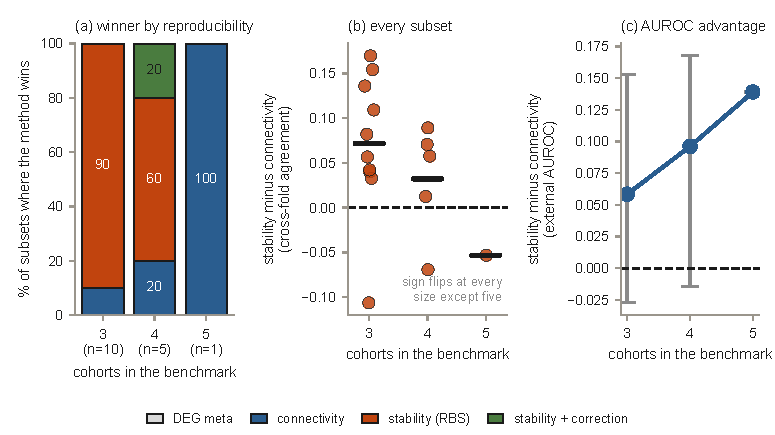
\includegraphics[width=\textwidth]{Fig2}
\caption{\textbf{Absolute AUROC is uninformative in this disease.} External AUROC for random
50-gene signatures, for permuted-label controls, and for the selected signatures, by held-out
cohort. Random signatures reach 0.68--0.88 depending on the fold; permuted labels sit at
approximately 0.50. A reported AUROC must be read against the random-signature band for its fold,
not against 0.5.}\label{fig:null}
\smallskip\noindent{\footnotesize Alt text: Dot plot of external AUROC by held-out cohort for three groups: random 50-gene signatures, permuted-label controls and the selected signatures. Random signatures form a band from about 0.68 to 0.88 that differs by fold; permuted labels sit near 0.50; the selected signatures are shown against that band for each fold.}
\end{figure}


\begin{table}[h]
\caption{Random-signature and permuted-label nulls, by held-out cohort ($K = 50$)}\label{tab:null}
\begin{tabular}{@{}lll@{}}
\toprule
Held out & Random 50-gene AUROC & Permuted labels \\
\midrule
GSE30528  & 0.682 [0.385--0.923] & 0.52 \\
GSE96804  & 0.796 [0.597--0.946] & 0.47 \\
GSE104948 & 0.809 [0.602--0.962] & 0.55 \\
GSE142025 & 0.878 [0.654--1.000] & 0.49 \\
\botrule
\end{tabular}
\footnotetext{Brackets give the 5th--95th percentile over 300 random draws.}
\end{table}

A comparable random-signature phenomenon appears in a metabolomic layer, measured in
different patients by a different principle. In plasma from ST003255 (64 diabetic
nephropathy, 66 IgA nephropathy, 66 membranous nephropathy, 24 hypertensive nephropathy,
66 healthy), randomly drawn 20-metabolite sets reach a cross-validated AUROC of 0.913
against healthy controls, while a set selected inside each fold reaches 0.995 and permuted
labels give 0.50. Imputation, log transformation and scaling are fitted on the training
fold only and applied to the held-out fold, so no test sample contributes to the transform.
The signature size was fixed at 20 in advance; at 10 the selected set still clears the 95th
percentile of the null and at 50 it no longer does, which is itself the point: the margin
over the null, not the absolute figure, is what a comparison can rest on. This is a single
cohort evaluated by cross-validation rather than an independent replication, and we read it
as a cross-modal illustration that the reporting problem is not confined to transcriptomes.

Every AUROC reported below is therefore accompanied by its position in this null.

\subsection{Reproducibility verdicts depend on cohort composition, not on
method}\label{sec:sensitivity}

Repeating the full benchmark over all subsets of the five discovery cohorts gives the
distribution of conclusions a study could have reported (Table~\ref{tab:sensitivity},
Fig.~\ref{fig:sensitivity}).

\begin{figure}[htbp]
% source: P1_cohort_sensitivity
\centering
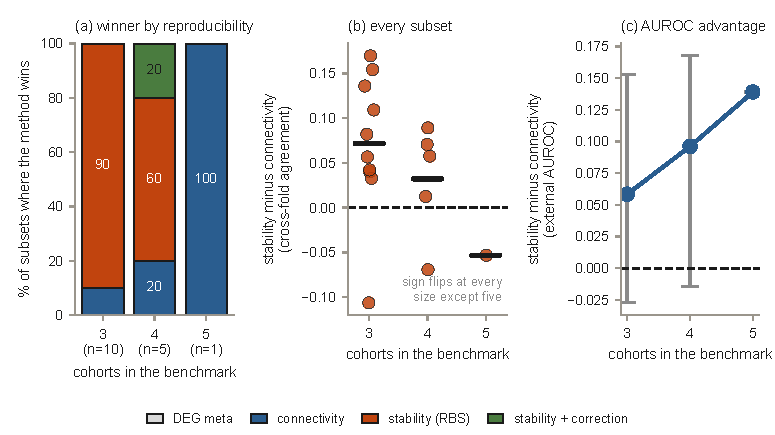
\includegraphics[width=\textwidth]{Fig3}
\caption{\textbf{The reproducibility verdict depends on which cohorts are benchmarked; the predictive advantage stays positive.} The benchmark was repeated over all 26 non-trivial subsets of the
five discovery cohorts; the panels show the 16 of size three or more. Two-cohort subsets are
excluded because they leave only two folds, so cross-fold agreement collapses towards zero and
ties between methods cannot be broken. \textbf{a} Percentage of subsets in which each method
wins on cross-fold reproducibility, by subset size, counting only subsets with a single top
scorer. \textbf{b} The same comparison shown for every individual subset: stability selection
minus the connectivity comparator in cross-fold agreement. The difference spans $-0.106$ to
$+0.170$ and changes sign at every subset size except five. Custom co-expression hub comparator; not the reference WGCNA implementation. \textbf{c} The same subsets scored by
external AUROC instead. Here the advantage is positive at every size and grows monotonically
($+0.058$, $+0.096$, $+0.139$ for sizes three through five). Reproducibility
and predictive performance are therefore not interchangeable summaries of the same
quantity.}\label{fig:sensitivity}
\smallskip\noindent{\footnotesize Alt text: Three panels. Left, stacked bars by benchmark size (three, four, five cohorts) of the percentage of subsets in which each selection method wins on cross-fold reproducibility. Middle, one point per subset of stability selection minus the connectivity comparator in cross-fold agreement, spanning minus 0.106 to plus 0.170 with points on both sides of zero at every size except five. Right, the mean external AUROC difference with its range, positive at every size.}
\end{figure}


\begin{table}[h]
\caption{Benchmark winner by cross-fold reproducibility, by subset size}\label{tab:sensitivity}
\begin{tabular}{@{}lll@{}}
\toprule
Cohorts & Subsets & Winner by reproducibility \\
\midrule
3 & 10 & RBS 9 (90\%), connectivity 1 (10\%) \\
4 & 5  & RBS 3 (60\%), connectivity 1 (20\%), RBS\_orth 1 (20\%) \\
5 & 1  & connectivity 1 (100\%) \\
\botrule
\end{tabular}
\end{table}

The paired difference RBS $-$ connectivity in cross-fold agreement spans $-0.106$ to $+0.170$ across
three-cohort subsets. The two extremes are concrete: a study using GSE96804 $+$ GSE142025 $+$
GSE294519 would report $+0.170$ in favour of stability selection, while one using GSE30528 $+$
GSE104948 $+$ GSE142025 would report $-0.106$ against it. Both are legitimate three-cohort DKD
benchmarks.

External AUROC behaves differently. Its advantage is directionally stable and grows with cohort
count: $+0.056$ (2 cohorts), $+0.058$ (3), $+0.096$ (4), and $+0.139$ at five cohorts. The
paired bootstrap put that five-cohort difference at $+0.129$ [$-0.002$, $+0.263$] ($p = 0.06$ over
200 replicates): the mean difference favoured stability selection, but the interval included zero.

The two metrics do not even agree on which method won. Excluding subsets where the top score is
tied, the method ranked first on cross-fold reproducibility is also the one ranked first on
external AUROC in 11 of 24 subsets. At three cohorts the two agree in 5 of 10. A benchmark
that reports one of these numbers is therefore not reporting a weaker version of the other.

The instability is not a property of one selector pair. Repeating the 26-subset sweep with each
of six further inner selectors of stability selection, against the same connectivity comparator,
reproduced it in every case (Table~\ref{tab:selectors}): the three-cohort reproducibility
difference changed sign under all seven selectors, in 1 to 5 of the 10 subsets, and with all five
cohorts the connectivity comparator won on reproducibility while stability selection won on
external AUROC under every selector. Random forest was the least stable, reversing in half of the
three-cohort subsets. What the seven share is the comparator and the cohorts, so the instability
belongs to the cohort set rather than to any selector, within the classical families tested.

The comparator side was checked the same way. Replacing the reimplementation by the WGCNA
package itself, run with its tutorial defaults on every fold (settings in the note to
Table~\ref{tab:selectors}), reproduced the reversal: the three-cohort difference spanned $-0.081$
to $+0.261$, and with all five cohorts the package won on reproducibility ($-0.133$) while
stability selection won on external AUROC ($+0.080$). The package was the weaker comparator on
both axes (mean Jaccard 0.064 and AUROC 0.711 over the 26 subsets, against 0.107 and 0.783 for
the reimplementation), so the reimplementation did not flatter stability selection.

\begin{table}[h]
\caption{Verdict instability under each inner selector of stability selection}\label{tab:selectors}
\footnotesize
\setlength{\tabcolsep}{3pt}
\begin{tabular}{@{}lrrrrrr@{}}
\toprule
Inner selector & Jaccard, 3 cohorts & Neg. & AUROC, 3 cohorts & Neg. & Jaccard, 5 & AUROC, 5 \\
\midrule
ReliefF (headline) & $-0.106$ to $+0.170$ & 1 & $-0.027$ to $+0.153$ & 2 & $-0.053$ & $+0.139$ \\
Univariate $F$     & $-0.111$ to $+0.150$ & 1 & $-0.098$ to $+0.150$ & 2 & $-0.063$ & $+0.101$ \\
LASSO              & $-0.127$ to $+0.119$ & 2 & $-0.112$ to $+0.146$ & 1 & $-0.090$ & $+0.078$ \\
Elastic net        & $-0.163$ to $+0.119$ & 2 & $-0.033$ to $+0.119$ & 1 & $-0.106$ & $+0.091$ \\
mRMR               & $-0.105$ to $+0.154$ & 1 & $-0.096$ to $+0.129$ & 2 & $-0.037$ & $+0.088$ \\
Random forest      & $-0.211$ to $+0.074$ & 5 & $-0.039$ to $+0.127$ & 3 & $-0.144$ & $+0.125$ \\
Boruta             & $-0.157$ to $+0.120$ & 2 & $-0.106$ to $+0.106$ & 3 & $-0.145$ & $+0.111$ \\
\midrule
\multicolumn{7}{l}{\textit{Comparator replaced by the WGCNA package (ReliefF inner selector)}} \\
WGCNA package      & $-0.081$ to $+0.261$ & 1 & $-0.007$ to $+0.283$ & 1 & $-0.133$ & $+0.080$ \\
\botrule
\end{tabular}
\footnotetext{Stability selection minus the connectivity comparator, the inner selector of stability selection varied; the comparator is unchanged. Ten three-cohort subsets per row; Neg., subsets in which the difference is negative. Five, the single five-cohort benchmark. Rows above the rule use the custom co-expression hub comparator, not the reference WGCNA implementation. The last row replaces the custom comparator by the WGCNA package run with its tutorial defaults on every fold (soft power by scale-free fit, 4--20 here; unsigned TOM; dynamic tree cut; module most correlated with the trait; hubs by $|$kME$|$).}
\end{table}

The practical consequence is that cross-fold agreement, the metric most often used to argue that
a selection method produces reproducible signatures, is the metric least able to support that
argument from a single cohort configuration. We therefore state what a benchmark on public
omics cohorts should report alongside its headline figure: the range of the method difference
over all admissible cohort subsets, whether that difference changes sign, how often each method
wins at a fixed subset size with ties excluded, and the two metrics side by side rather than
one standing for both. The patient-overlap audit and the control-procurement table are inputs to
that protocol, not preliminaries to it. Without the overlap audit, the independence of
admissible subsets cannot be assessed; without the control-procurement table, their
sensitivity cannot be interpreted as a design finding. Table~\ref{tab:checklist} collects these items, together with the controls the later sections add, as the checklist we recommend.

\begin{table}[h]
\caption{What a cross-cohort feature-selection benchmark on public cohorts should report, and where each item is applied here}\label{tab:checklist}
\footnotesize
\setlength{\tabcolsep}{4pt}
\begin{tabular}{@{}p{46mm}p{46mm}p{28mm}@{}}
\toprule
Report & Because & Here \\
\midrule
The method difference as a range over all admissible cohort subsets & a single configuration is one draw from that range & Section~\ref{sec:sensitivity} \\
Whether that difference changes sign across subsets & a sign change makes the verdict a statement about the cohorts & Section~\ref{sec:sensitivity} \\
Winner frequency at a fixed subset size, ties excluded & with few folds, ties inflate apparent wins & Section~\ref{sec:sensitivity} \\
Reproducibility and predictive performance side by side & the two agreed on the winner in only 11 of 24 subsets & Section~\ref{sec:sensitivity} \\
Every AUROC with its position in a random-signature null & random 50-gene sets reached 0.68--0.88 & Section~\ref{sec:auroc-null} \\
A patient-overlap audit across accessions & reused patients make subsets and folds non-independent & Section~\ref{sec:cohorts} \\
Procurement route of cases and of controls, per cohort & collinearity with diagnosis is a design confounder no selector can remove & Section~\ref{sec:procurement} \\
A confounder-matched contrast wherever one exists & it did more work here than any algorithm & Sections~\ref{sec:whichcorrections}, \ref{sec:external} \\
Pre-analytical variables to the SPREC or BRISQ standard & they turn the inference into a measurable covariate & unavailable in every cohort used \\
\botrule
\end{tabular}
\end{table}

\subsection{The most reproducible signal tracks tissue procurement, not
disease}\label{sec:procurement}

\textbf{A note on what is and is not measured.} No DKD cohort we examined reports warm or cold
ischaemia time, fixation, or time to stabilisation. Procurement route is read from the sample
source annotation (needle biopsy versus nephrectomy or donor tissue), so the attribution to
pre-analytical handling is an inference, not a measurement. It rests on three things: the
association between procurement route and module level holds across nine datasets and four
platforms; the module does not separate two groups that share a procurement route, even when one
is diabetic and the other is not; and warm ischaemia is independently documented to induce
exactly these transcripts within minutes, including in kidney \cite{ma2012}, and ischaemia time is a documented driver of transcriptome variation across human tissues at scale \cite{ferreira2018}. Since this analysis was completed, an independent single-cell comparison of reference tissue sources within KPMP has reported the same dependence: stress-response genes are higher in nephrectomy and living-donor tissue than in percutaneous biopsies from healthy volunteers, and the choice of reference changes which genes are called differentially expressed \cite{menon2026}. We use
``procurement-associated'' throughout and reserve ``artifact'' for the interpretation, which the
data support but do not prove.

Across nine kidney datasets the IEG module tracks how tissue was obtained, not disease
(Table~\ref{tab:procurement}, Fig.~\ref{fig:procurement}). The Spearman correlation between
procurement (biopsy versus non-biopsy) and module level across all groups is $\rho = -0.752$,
$p < 0.001$.

\begin{figure}[htbp]
% source: P3_procurement
\centering
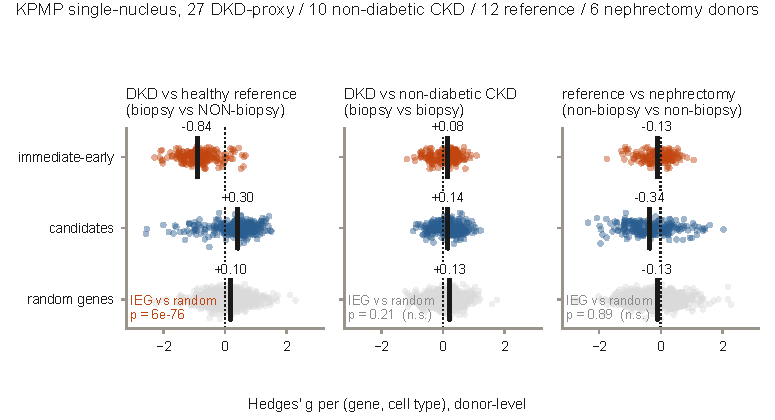
\includegraphics[width=\textwidth]{Fig4}
\caption{\textbf{The most reproducible signal tracks tissue procurement, and it is
organ-specific.} \textbf{a} The immediate-early gene module, $z$-scored within dataset, for every
diagnosis group in nine kidney datasets, ordered by effect. Biopsy-procured groups sit below
nephrectomy- and donor-procured groups in eight of the nine (Spearman $\rho = -0.75$,
$p < 0.001$); GSE162830, the one histology-matched design, is the exception. \textbf{b} The same
module as Hedges' $g$ for four contrasts. In KPMP, DKD against non-biopsy reference tissue gives
$-0.84$ while DKD against other biopsies gives $+0.08$. In the heart-failure cohort GSE5406,
disease against donor reaches only $-0.23$ and the within-procurement contrast (ischaemic against
idiopathic) is $+0.33$. The kidney effect therefore appears when procurement differs and vanishes
when it does not, and it does not transfer to heart, which bounds the claim to kidney procurement
rather than to tissue injury in general.}\label{fig:procurement}
\smallskip\noindent{\footnotesize Alt text: Two panels. Left, a dumbbell chart of nine kidney datasets in which biopsy-procured groups (orange) sit below nephrectomy- or donor-procured groups (blue) on the immediate-early module score in eight of nine; GSE162830 shows no gap. Right, horizontal bars of Hedges g for four contrasts: in KPMP, diabetic kidney disease against non-biopsy reference tissue minus 0.84 and against other biopsies plus 0.08; in heart failure, disease against donor minus 0.23 and ischaemic against idiopathic plus 0.33.}
\end{figure}


\begin{table}[h]
\caption{Immediate-early module level by procurement route, across nine kidney
datasets}\label{tab:procurement}
\begin{tabular}{@{}llll@{}}
\toprule
Dataset & Biopsy & Non-biopsy & Difference \\
\midrule
GSE142025  & $-0.63$ & $+1.26$ & $-1.90$ \\
GSE104954  & $-0.23$ & $+1.37$ & $-1.60$ \\
GSE175759  & $-0.21$ & $+1.10$ & $-1.31$ \\
GSE96804   & $-0.39$ & $+0.80$ & $-1.19$ \\
GSE104948  & $-0.15$ & $+0.88$ & $-1.03$ \\
KPMP snRNA & $-0.33$ & $+0.64$ & $-0.97$ \\
GSE30529   & $-0.26$ & $+0.22$ & $-0.48$ \\
GSE30528   & $-0.19$ & $+0.13$ & $-0.32$ \\
GSE162830  & $+0.13$ & $+0.18$ & $-0.05$ \\
\botrule
\end{tabular}
\footnotetext{Values are the module mean $z$-score computed within each dataset.}
\end{table}

The KPMP single-nucleus data provide the decisive control because they contain both contrasts
with donor-level replication (27 DKD-proxy donors as defined in Section~\ref{sec:cohorts}, 10 non-diabetic CKD, 12 reference, 6 nephrectomy donors;
statistics on donor $\times$ cell-type pseudobulk, Fig.~\ref{fig:singlecell}; the three
contrasts are tabulated in Additional file~4).

\begin{figure}[htbp]
% source: P4_singlecell_control
\centering
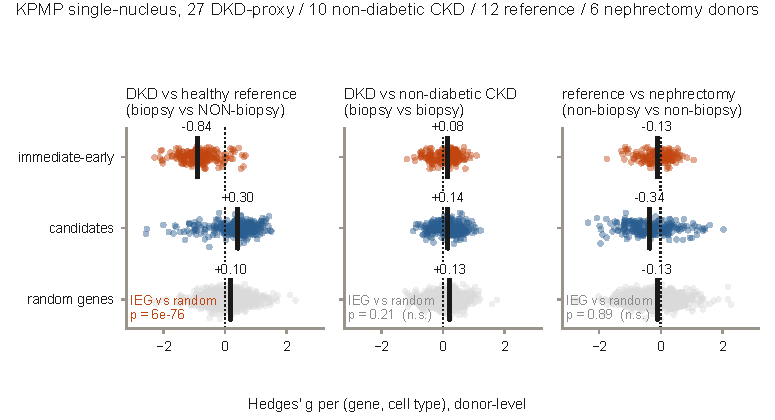
\includegraphics[width=\textwidth]{Fig5}
\caption{\textbf{A biopsy-versus-biopsy contrast removes the effect.} KPMP single-nucleus data
reduced to donor-level pseudobulk. Comparing DKD with non-diabetic CKD, both procured by needle
biopsy, gives $p = 0.21$; comparing DKD with non-biopsy reference tissue in the same resource
gives $p = 6.0\times10^{-76}$. The contrast is the negative control for
Fig.~\ref{fig:procurement}: when procurement is held constant the signal disappears, and it is
not a property of DKD.}\label{fig:singlecell}
\smallskip\noindent{\footnotesize Alt text: Box plots of the immediate-early module score in KPMP single-nucleus pseudobulk by donor. Diabetic kidney disease against non-diabetic chronic kidney disease, both needle biopsies, shows overlapping distributions (p equals 0.21); diabetic kidney disease against non-biopsy reference tissue shows a clear separation.}
\end{figure}


GSE162830, the single dataset where all 32 samples were processed identically (OCT,
$-80\,^{\circ}$C, laser microdissection), shows no procurement effect at all ($-0.05$), which is
what the interpretation predicts.

Because cases are biopsies and controls surgical tissue in every discovery contrast, this
confounder is shared across cohorts and therefore maximally reproducible. A criterion that
rewards cross-cohort consistency will rank it first: uncorrected RBS places 10 immediate-early
genes in its top 50.

This is organ- and protocol-specific, not universal, and we report it in the main text rather
than as supplementary material because it bounds the claim. In heart failure (GSE5406, 194
explanted ventricles versus 16 donor hearts) the module separates explant from donor only weakly
($g = -0.23$) and instead separates ischaemic from idiopathic cardiomyopathy, both explants
($p = 4\times10^{-8}$). Explanted and donor hearts undergo similar cardioplegia and cold storage,
whereas needle biopsies and nephrectomies differ substantially in warm ischaemia. The confounder
is a property of the procurement contrast, not of the gene module.

\subsection{Why one method escaped the confounder, and why that is not
robustness}\label{sec:modulesize}

This section exists to close a loophole in Section~\ref{sec:procurement} rather than to open a
second topic. If a widely used criterion simply avoids the confounder, the problem is less
serious than we claim. It does avoid it here, but for a reason that does not generalise.

The connectivity comparator placed no immediate-early genes in its top 50 while stability
selection placed 10. This exclusion alone does not establish robustness. In the real data 12 of 19 immediate-early genes are inside the disease-correlated
module and have high gene--trait correlation (\textit{DUSP1} $|gs| = 0.710$, among the highest in
the module), yet rank 790th of 990 by connectivity, because intramodular connectivity is a
\emph{sum} of adjacencies and therefore rewards membership of the largest coherent block: the
median block size (module genes with $|r| > 0.5$) is 19 for the immediate-early genes against 705
for the top 50 by connectivity, and 395 for the whole module.

This is not an artifact of how the comparator was implemented. Rebuilding it across every
combination of module definition (gene--trait correlation or clustering on the topological
overlap matrix), hub criterion (intramodular connectivity or module membership), adjacency
(signed or unsigned) and soft power ($\beta \in \{4, 6, 8, 12\}$, spanning both our value and
the $\beta \ge 10$ the scale-free criterion would select on these data) gives 32 variants, and
\emph{all 32 place no immediate-early gene in the top 50}. The WGCNA package itself, run with its
tutorial defaults on every fold of the cohort sweep, does not: in 9 of 75 folds (3 of the 30 distinct training combinations the folds evaluate) it
placed immediate-early genes in its top 50, up to 18 of 50, always where dynamic tree cut had
produced a small trait module (61 to 199 genes against a median of 588). Because the package ranks
by $|$kME$|$ within the chosen module, this is consistent with module-dependent exclusion rather
than a direct test of the summed-connectivity account; the median rank of an immediate-early
gene within its module ranges from 664 to 3{,}531. Under a signed network the immediate-early
genes are not module members at all, so the confounder is missed earlier still. Raising $\beta$
improves their rank without approaching the top 50, so our lower $\beta$ is conservative against
our own argument. Additional file~1 reports the full grid.

Simulation confirms the mechanism and shows that it reverses (Fig.~\ref{fig:blocksize}; the
paired differences are tabulated in Additional file~1).

\begin{figure}[htbp]
% source: P5_block_size
\centering
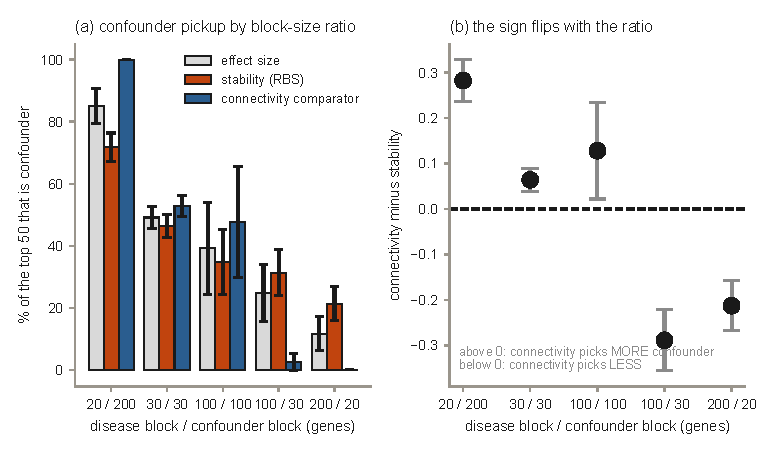
\includegraphics[width=\textwidth]{Fig6}
\caption{\textbf{Connectivity criteria are biased by module size, which is why one method
escaped.} Simulation sweeping the ratio between the size of the disease block and that of the
confounder block. \textbf{a} Percentage of the top 50 features that come from the confounder
block. \textbf{b} The difference between a connectivity criterion and a stability criterion,
which changes sign as the ratio crosses one. In the real data the immediate-early block contains
19 genes against 705 in the top-connectivity block, placing it in the regime where connectivity
misses the confounder for reasons unrelated to robustness. All seven configurations are
significant by Wilcoxon signed-rank on paired replicates.}\label{fig:blocksize}
\smallskip\noindent{\footnotesize Alt text: Two line panels over the ratio of disease-block size to confounder-block size in a simulation. Left, the percentage of the top 50 features drawn from the confounder block for each criterion as the ratio changes. Right, the difference between the connectivity and stability criteria, crossing zero where the ratio equals one. A marker shows the real-data regime, 19 immediate-early genes against 705 top-connectivity genes.}
\end{figure}


The sign tracks the block-size ratio; effect-size and stability criteria show no such dependence
(differences $-0.025$ to $+0.022$ across the same configurations). The connectivity comparator avoided the kidney
confounder because that confounder happened to form a small block. Where a confounder forms a
large programme, connectivity is the worst of the three.

\subsection{Which corrections work}\label{sec:whichcorrections}

Corrections are compared on three axes at once: how much of the confounder survives, whether the
surviving signal is DKD-specific, and what the correction costs in external AUROC
(Table~\ref{tab:corrections}, Fig.~\ref{fig:corrections}).

\begin{figure}[htbp]
% source: P6_corrections
\centering
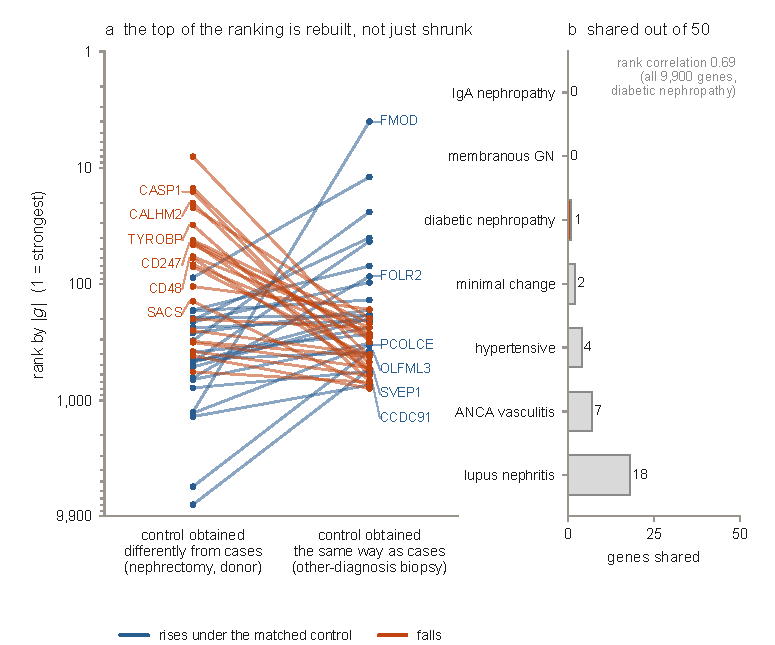
\includegraphics[width=\textwidth]{Fig7}
\caption{\textbf{What each correction removes, and what it costs.} \textbf{a} Percentage of the
top 50 selected features flagged as procurement-driven, lower being better. \textbf{b}
Specificity pass-rate expressed as fold-enrichment over the 8.3\% background rate at which a
random gene passes the gate, so that no bar can be read as an absolute success rate. \textbf{c}
External AUROC, showing the cost of correcting. Handling-score residualisation and
surrogate-variable analysis reduce procurement-driven features from 27\% to 5--6\%; residualisation
does so at a fold-mean AUROC identical to no correction to three decimal places, surrogate-variable
analysis at 0.915 against 0.926. The separate paired bootstrap estimate of the residualisation cost
is uncertain and is given in the text. ComBat returned the same values as no correction in this
evaluation setting; the confounder is within-cohort rather than between-cohort.}\label{fig:corrections}
\smallskip\noindent{\footnotesize Alt text: Three panels of horizontal bars for six correction strategies. Left, the percentage of the top 50 selected features flagged as procurement-driven: 27 percent with no correction or ComBat, 5 to 6 percent with handling-score residualisation or surrogate-variable analysis. Middle, specificity pass rate as fold enrichment over the 8.3 percent background. Right, external AUROC, 0.926 for no correction and residualisation and 0.915 for surrogate-variable analysis.}
\end{figure}


\begin{table}[h]
\caption{Correction benchmark at $K = 50$}\label{tab:corrections}
\begin{tabular}{@{}llllll@{}}
\toprule
Correction & IEG in top 50 & Procurement- & Specificity & AUROC & Cross- \\
           &               & flagged      & pass        &       & fold \\
\midrule
None                            & 8.5 & 27\% & 33\% & 0.926 & 0.284 \\
ComBat (batch $=$ cohort)       & 8.5 & 27\% & 33\% & 0.926 & 0.284 \\
RUVg, empirical controls        & 7.5 & 28\% & 26\% & 0.924 & 0.154 \\
RUVg, module as controls        & 0.8 & 18\% & 40\% & 0.905 & 0.215 \\
Surrogate-variable adjustment   & 2.0 & 6\%  & 44\% & 0.915 & 0.251 \\
Residualise on handling score   & 1.0 & 5\%  & 40\% & 0.926 & 0.260 \\
\botrule
\end{tabular}
\footnotetext{Specificity pass is the fraction of selected genes clearing the DKD-versus-other-CKD
gate. Two rates are involved and they have different denominators. The \emph{background pass rate} is 8.3\%: 820 of the 9,900 genes in the frozen space clear the gate, so a random set clears it at that rate and the 40--44\% figures are approximately $5\times$ background. The gate's \emph{permutation-based false-discovery estimate} is 16.7\%: of those 820 passers, 137 are expected when the labels are permuted. The two ERCB blocks profile the same patients in two compartments, so the labels are permuted at the patient level; shuffling each block independently returns 13.7\%, which understates the gate because it removes a dependence the real data has.}
\end{table}

ComBat returns the same values as no correction in this implementation and evaluation setting.
Cohort-level batch adjustment alone cannot disentangle procurement from disease when the two are
confounded \emph{within} cohorts. RUVg with
empirically chosen controls also fails; the control set, not the framework, does the work.
Residualisation and surrogate-variable adjustment both succeed. Table~\ref{tab:corrections}
reports identical fold-mean AUROCs to three decimal places for no correction and for
residualisation. In a separate patient-stratified paired bootstrap analysis with 200 replicates,
which resamples patients within each cohort and class and re-runs the whole leave-one-dataset-out
evaluation in every replicate at a reduced inner bootstrap ($B = 30$ rather than the 150 of the
fold means), the mean uncorrected minus residualised difference was $+0.079$ (95\% percentile
interval $-0.048$ to $+0.229$). This exploratory uncertainty estimate does not establish
performance preservation: a substantial loss remains compatible with the interval, whose tails are
imprecisely estimated.

The evaluation is not circular: the procurement flag derives from ERCB effect sizes, not from
module membership, and correlation with the handling score separates flagged from unflagged genes
at AUC $= 0.480$ (0.5 indicates independence).

The correction is not specific to the selector it was benchmarked with. Repeating the comparison with each of the seven inner selectors of Section~\ref{sec:selectors}, at $B = 40$ rather than 150 because the question is the direction of the change rather than its third decimal, the procurement-flagged fraction of the top 50 falls for every one of them (Table~\ref{tab:sweep}), from 17.0--35.5\% to 3.5--12.5\%. The cost is not uniform. External AUROC rises for ReliefF (+0.021), falls by less than 0.05 for Boruta and mRMR, and falls by 0.05 to 0.11 for Elastic net, LASSO, Random forest and Univariate $F$. The removal is therefore a property of the correction, its cost a property of the selector, and a study adopting the correction should report that cost for the selector it uses.

\begin{table}[h]
\caption{The handling-score correction under each inner selector ($K = 50$, $B = 40$): procurement-flagged share of the selected features and external AUROC, uncorrected and corrected}\label{tab:sweep}
\begin{tabular}{@{}lrrrrr@{}}
\toprule
Selector & Flagged, & Flagged, & AUROC, & AUROC, & Change \\
         & uncorrected & corrected & uncorrected & corrected & in AUROC \\
\midrule
Univariate $F$ & 24.5\% & 6.0\% & 0.921 & 0.807 & -0.114 \\
LASSO & 33.0\% & 12.5\% & 0.956 & 0.879 & -0.077 \\
Elastic net & 35.5\% & 3.5\% & 0.909 & 0.857 & -0.052 \\
mRMR & 28.0\% & 6.5\% & 0.941 & 0.896 & -0.046 \\
ReliefF & 29.5\% & 5.0\% & 0.928 & 0.949 & +0.021 \\
Random forest & 17.0\% & 7.5\% & 0.895 & 0.815 & -0.079 \\
Boruta & 22.0\% & 6.5\% & 0.918 & 0.901 & -0.017 \\
\botrule
\end{tabular}
\footnotetext{Each row is the mean over leave-one-dataset-out folds on the four headline cohorts. The ReliefF row repeats the comparison of Table~\ref{tab:corrections} at the lower $B$; the small differences between the two rows are the bootstrap resolution, not a change in method.}
\end{table}

\subsection{The control-group problem is not specific to diabetic kidney
disease}\label{sec:external}

Everything above concerns one disease, which leaves open whether the effect is a property of
diabetic kidney disease or of the design that every public kidney biopsy study shares. The ERCB
compartments answer this inside a single resource, because they contain eight biopsy diagnoses
alongside the same non-biopsy controls. We call the comparison that follows a \emph{control-
definition sensitivity analysis}: holding the case set fixed, it asks how far the ranking and
the effect-size conclusions move when the control group is replaced by an alternative that is
clinically defensible. It does not separate clinical from pre-analytical causes, and we do not
claim it does; procurement is our reading of why the two definitions differ here, supported
by the evidence in Section~\ref{sec:procurement} rather than established by this comparison. For each diagnosis we formed the two contrasts the
argument turns on, namely diagnosis versus non-biopsy control and diagnosis versus the
remaining biopsy diagnoses, and counted genes reaching $|g| \ge 0.5$ (Table~\ref{tab:ckdgen}). Seven of the
eight are reported; thin membrane disease was left out because its 9 cases give neither
contrast usable power.

\begin{table}[h]
\caption{Genes at $|g| \ge 0.5$ before and after matching the control group, by
diagnosis}\label{tab:ckdgen}
\begin{tabular}{@{}lrrrr@{}}
\toprule
Diagnosis & Patients & vs non-biopsy & vs other biopsy & Median $|g|$ \\
\midrule
IgA nephropathy               & 52 & 3{,}800 & 0     & 14\% \\
Systemic lupus erythematosus  & 65 & 4{,}506 & 166   & 30\% \\
Hypertensive nephropathy      & 35 & 3{,}251 & 9     & 30\% \\
Diabetic nephropathy          & 29 & 5{,}107 & 833   & 37\% \\
ANCA-associated vasculitis    & 43 & 5{,}878 & 1{,}981 & 42\% \\
Minimal change disease        & 27 & 3{,}351 & 690   & 54\% \\
Membranous glomerulonephropathy & 38 & 3{,}282 & 702 & 56\% \\
\botrule
\end{tabular}
\footnotetext{The last column is the ratio of median $|g|$ under the matched contrast to median $|g|$
under the naive one, a retained effect size rather than a retained count of genes, so it is
not sensitive to the differing group sizes. All seven Wilcoxon
tests on the paired effect vectors give $p < 10^{-300}$.}
\end{table}

Shrinking is not the whole of it. A signal that fell uniformly would leave the ranking, and
therefore the candidate list, unchanged; what happens instead is that the top of the ranking is
rebuilt (Figure~\ref{fig:reordering}). Taking the 50 largest effects under each contrast, the two
lists share 1 gene in diabetic nephropathy and between 0 and 18 across the seven
diagnoses. The comparison holds the case set fixed and varies the control group; it is not
a within-patient pairing, for which no public data exist. Rank correlation over all 9,900 genes is 0.69 for diabetic
nephropathy, so the bulk of the transcriptome moves together while the extreme that feeds
selection does not. The movement has direction: myeloid and inflammatory genes fall (\textit{TYROBP}
31 to 678, \textit{CASP1} 16 to 603) while matrix genes rise (\textit{FMOD} 1264 to 4,
\textit{OLFML3} 5530 to 377). \textit{MOXD1} moves from 204 to 40; that is a change in
priority under a contrast with less procurement asymmetry, not evidence that it is a marker.

\begin{figure}[htbp]
% source: P9_reordering
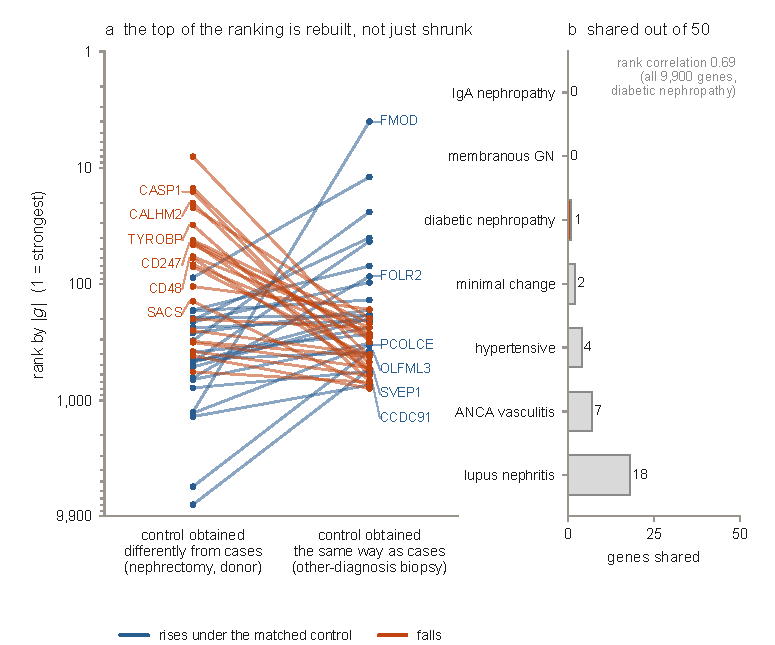
\includegraphics[width=\textwidth]{Fig8}
\caption{\textbf{Changing the control-group definition rebuilds the top of the ranking.}
\textbf{a} Each line is one gene, drawn between its rank by $|g|$ when diabetic nephropathy
cases are compared with non-biopsy controls (left) and its rank when the same cases are
compared with biopsies of other diagnoses (right). Blue rises under the matched control,
orange falls. The 46 genes drawn are those reaching either candidate list; 23 rise and 23 fall.
Rank is on a log scale because the difference between first and twentieth matters for
selection and the difference between five thousandth and five thousand five hundredth does
not. \textbf{b} Genes shared by the two top-50 lists, computed over all 9,900 genes rather
than the subset drawn in \textbf{a}, for each of the seven ERCB biopsy diagnoses. This is the same case
set compared against two control groups, not a within-patient pairing; no public resource
provides the latter. \textit{MOXD1} rising from 204 to 40 is a change in priority under a
contrast with less procurement asymmetry, not evidence that it is a marker.}\label{fig:reordering}
\smallskip\noindent{\footnotesize Alt text: Two panels. Left, a slope chart of 46 genes drawn between their rank against non-biopsy controls and their rank against other-diagnosis biopsies in diabetic nephropathy, on a logarithmic rank axis; blue lines rise under the matched control and orange lines fall, 23 each. Right, horizontal bars of the number of genes shared by the two top-50 lists for seven ERCB biopsy diagnoses.}
\end{figure}


The consequence for a candidate list is direct. Running the same pipeline with and without
the handling-score correction returns 30 candidates each, sharing only 14
(Additional file~3). Which genes a study nominates is therefore set by how its control
tissue was obtained as much as by the disease.

Every diagnosis loses most of its signal, and diabetic nephropathy is unremarkable among them:
it ranks fourth of seven, and the median across the other six is 36\% against its 37\%. In IgA
nephropathy the 3,800 genes reaching $|g| \ge 0.5$ against non-biopsy controls fall to none.
The problem therefore belongs to the design rather than to the disease, and the argument of
Sections~\ref{sec:procurement} and~\ref{sec:whichcorrections} applies to kidney biopsy studies
generally. One qualification carries over from Section~\ref{sec:procurement}: the matched
comparator here pools the remaining diagnoses, and pooling can itself produce a result, so these
figures should be read as the pooled-comparator case.

Three datasets never used elsewhere in this work provide external checks of the candidate list.
In GSE20602, which compares nephrosclerosis glomeruli against tumour nephrectomy, the same
control type as GSE30528, the candidates move further in the diabetic contrast than in the
nephrosclerosis one (median $|g_{\text{DKD}}| - |g_{\text{NSC}}|$ of $+1.02$ against $-0.17$ for
the remaining genes, Mann--Whitney $p = 5.1 \times 10^{-18}$), which replicates the specificity
gate outside ERCB. In GSE111154 the candidates are already altered in early diabetic nephropathy
(permutation $p = 0.0015$), though with four patients per group this is weak. In GSE142153, blood
from diabetic nephropathy patients, the candidates are indistinguishable from random genes
($p = 0.80$): the signature is tissue-restricted, which supports its specificity and limits its
clinical accessibility at the same time.

The comparator behaves the same way in that metabolomic layer, which is the clearest
evidence that the recommendation is not specific to transcriptomics. Replacing the healthy
controls of ST003255 with the non-diabetic kidney disease patients of the same study drops the
random-set AUROC from 0.913 to 0.724, and the selected set clears its null by a wider
margin: 0.854 against a 95th percentile of 0.800, where against healthy controls it was
0.995 against 0.977. The reason is visible in the effect sizes. Across the 187 named metabolites the
diabetic-versus-healthy and other-kidney-disease-versus-healthy effect vectors correlate at
$r = 0.851$, so most of what separates these patients from healthy people is shared with kidney
disease in general. Twenty-nine metabolites survive the matched contrast at $q < 0.05$. A
disease-relevant comparator distinguishes diabetic-kidney-disease-associated changes from
metabolic changes shared across kidney diseases; it does not establish the procurement
mechanism seen in the transcriptome cohorts, which is a property of how those tissues
were obtained and has no counterpart in plasma.

\subsection{Both mechanisms outside kidney: predictions fixed before the
data}\label{sec:xtissue}

Section~\ref{sec:external} showed that the control-group problem is not specific to diabetic
nephropathy, but every diagnosis it could test was a kidney biopsy diagnosis. Whether verdict
instability and a reproducible procurement confounder belong to cross-cohort benchmarking or to
kidney cohorts needs tissues designed differently. Three predictions were fixed before any liver
or colon expression value was read (Section~\ref{sec:xtmethods}), and each verdict below is
judged against its written wording (Table~\ref{tab:xtissue}, Fig.~\ref{fig:xtissue}). The
analyses that followed the verdicts were stated before they ran and are reported as post hoc.

\begin{figure}[htbp]
% source: P10_cross_tissue
\centering
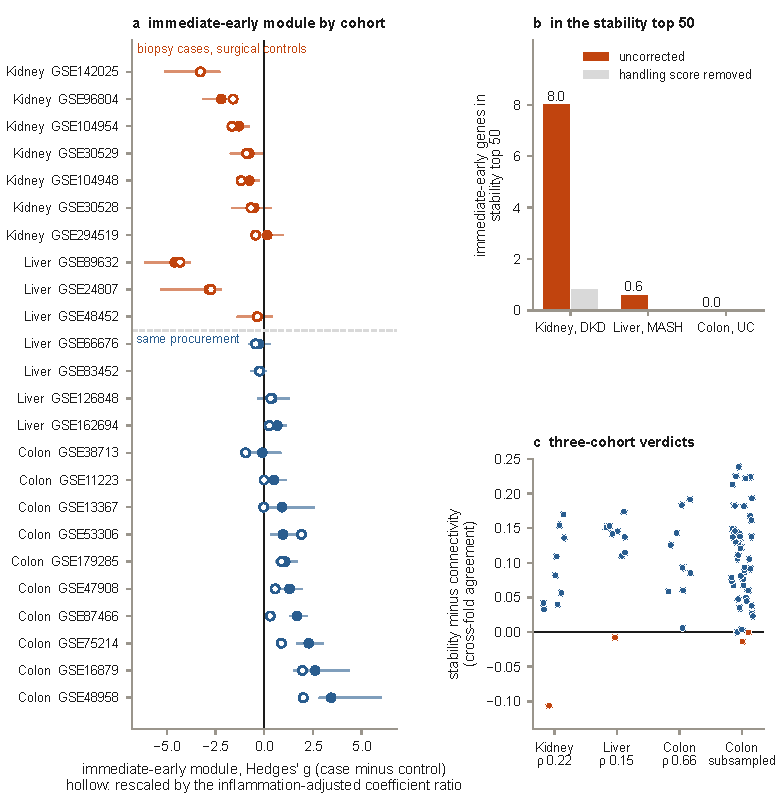
\includegraphics[width=\textwidth]{Fig9}
\caption{\textbf{Outside kidney, the module follows procurement where asymmetric and inflammation where matched.} \textbf{a}
Hedges' $g$ of the handling score, case minus control, with 95\% bootstrap intervals, for every
cohort whose procurement could be coded. Above the dashed line, biopsy cases against surgical or
donor controls; below, both arms obtained by the same procedure. Hollow points are not a second $g$: they are that $g$
multiplied by the ratio of the adjusted to the unadjusted standardised case coefficient from the
inflammation regression, which carries the adjustment onto the same axis. The two coefficients on
their own scale are in Additional file~7. \textbf{b} Mean number of immediate-early genes in the
stability-selection top 50 over leave-one-dataset-out folds on each tissue's five core cohorts,
uncorrected and after residualising on the handling score. \textbf{c} Stability selection minus
the connectivity comparator in cross-fold agreement for every three-cohort subset; orange points
are subsets in which the verdict reversed. Custom co-expression hub comparator; not the reference WGCNA implementation. $\rho$ is the median pairwise Spearman correlation of
gene-wise effect sizes across the five core cohorts. The rightmost column repeats colon with each
cohort subsampled to kidney case and control counts (five replicates of ten subsets). Filled
points in \textbf{a}, panel \textbf{b} and the first three columns of \textbf{c} test the
registered predictions; the inflammation adjustment, concordance and subsampling are post
hoc.}\label{fig:xtissue}
\smallskip\noindent{\footnotesize Alt text: Three panels. Left, a dot plot of Hedges g for the handling score, case minus control, with 95 percent bootstrap intervals, one row per cohort, split into cohorts with biopsy cases against surgical or donor controls (above the dashed line) and cohorts with both arms obtained by the same procedure (below); hollow points show the inflammation-adjusted value. Middle, bars of the mean number of immediate-early genes in the stability-selection top 50 per tissue, with and without correction. Right, per-subset reproducibility differences for kidney, liver and colon with reversed verdicts highlighted.}
\end{figure}


\begin{table}[h]
\caption{Predictions fixed before the liver and colon data were read, with the kidney reference computed by the same code}\label{tab:xtissue}
\footnotesize
\setlength{\tabcolsep}{3pt}
\begin{tabular}{@{}>{\raggedright\arraybackslash}p{36mm}>{\raggedright\arraybackslash}p{22mm}>{\raggedright\arraybackslash}p{22mm}>{\raggedright\arraybackslash}p{22mm}>{\raggedright\arraybackslash}p{18mm}@{}}
\toprule
Prediction & Kidney, DKD & Liver, MASH & Colon, UC & Verdict \\
\midrule
P1. The three-cohort RBS $-$ connectivity difference in cross-fold agreement spans zero & $-0.106$ to $+0.170$ (1 of 10 negative) & $-0.008$ to $+0.174$ (1 of 10) & $+0.006$ to $+0.192$ (0 of 10) & held in liver, failed in colon \\
\quad and the external AUROC difference changes sign in fewer subsets & $-0.027$ to $+0.153$ (2 of 10) & $+0.040$ to $+0.377$ (0 of 10) & $-0.005$ to $+0.067$ (1 of 10) & \\
P2. $|g_{\text{IEG}}| < 0.5$ in procurement-matched cohorts; negative, and larger than in every matched cohort, where cases are biopsies and controls surgical & 7 asymmetric, 6 negative & 3 asymmetric, all negative; 3 of 4 matched below 0.5 & 10 matched, 1 below 0.5, 9 positive & failed in both \\
P3. Immediate-early genes in the uncorrected stability top 50: kidney $>$ liver $>$ colon, colon at most 1; correction reduces the count substantially only in kidney & 8.0 (7.2 removed) & 0.6 (0.6 removed) & 0.0 & held \\
\botrule
\end{tabular}
\footnotetext{Wording abbreviated from the registered file (Additional file~7). The single negative liver subset recurs under five bootstrap seeds ($-0.017$ to $-0.008$), and the other nine stay positive in all five. Kidney values are a reference, not part of any prediction. By the same per-subset count the second clause of P1 would not hold in kidney either (2 AUROC sign changes against 1); the stability of the predictive verdict in Section~\ref{sec:sensitivity} rests on the mean advantage per subset size, which is positive at every size in all three tissues. The kidney P3 count is a mean over folds at the sweep's inner $B$, and so differs from the 10 of Section~\ref{sec:modulesize}.}
\end{table}

\textbf{Verdict instability (P1).} In liver the difference in cross-fold agreement between
stability selection and the connectivity comparator ranged from $-0.008$ to $+0.174$ across the ten
three-cohort subsets, crossing zero in one of the ten subsets tested and narrowly, while the
external AUROC difference stayed positive in all ten. That one reversal is small, so we asked
whether it is an artefact of the resampling seed. Repeating the ten three-cohort comparisons under
five bootstrap seeds reproduced it in the same subset (GSE89632 $+$ GSE48452 $+$ GSE83452) every
time, at $-0.017$ to $-0.008$, while the other nine subsets stayed positive under all five seeds.
The fifty runs are repeated computations on one dataset rather than fifty independent tests, so
this supports robustness to computational randomness and says nothing about patient-sample
uncertainty. P1 therefore holds in liver with that scope: a small reversal, repeatable, in one
configuration of ten. In colon the agreement difference never crossed zero ($+0.006$ to
$+0.192$), and the prediction failed there. Post hoc, the tissues differed most in how far their
cohorts agree about the disease: the median pairwise correlation of gene-wise effect sizes
across the five core cohorts was 0.66 in colon against 0.22 in kidney and 0.15 in liver. Cohort
size does not account for the difference. With each colon cohort subsampled to the case and
control counts of a kidney cohort, concordance stayed between 0.60 and 0.65 in five replicates,
and the agreement difference crossed zero in two of them, by at most 0.013, against a stated
threshold of three (Fig.~\ref{fig:xtissue}c). The sign changes of
Section~\ref{sec:sensitivity} were therefore associated with cohorts that disagree about the
disease signal rather than with cohort size, which three tissues cannot raise to a necessary
condition.
Concordance can be computed before any selection method is run, and a low value warns that a
single-configuration verdict is unlikely to transfer; three tissues are too few to treat it as a
threshold.

\textbf{The module at the cohort level (P2).} Where cases were needle biopsies and controls were
surgical or donor tissue, the immediate-early score was lower in cases in 9 of 10 cohorts across
the two tissues, with liver GSE89632 at $g = -4.60$ [$-6.11$, $-3.82$] and GSE24807 at
$-2.83$, both above the 99th percentile of random modules. The prediction nonetheless failed,
because matched cohorts were not near zero. In colon, where both arms are endoscopic biopsies,
the score was higher in inflamed cases in 9 of 10 cohorts ($+0.51$ to $+3.43$). In matched
liver cohorts it was small in three of four ($-0.28$ to $+0.40$; GSE162694 $+0.67$), and in
GSE48452, whose case arm mixes needle and intraoperative biopsies, it was $-0.37$. The module is
therefore not a pure procurement readout: it also responds to active inflammation. Adjusting for
the inflammation score shrank the colon case effect by a median of 49\% and left every
biopsy-versus-surgical cohort negative, all ten after adjustment against nine before (median
standardised coefficient $-0.94$ before and $-1.14$ after; matched cohorts $+0.89$ and
$+0.30$; Mann--Whitney $p = 1.6 \times 10^{-4}$ between the groups after adjustment). The
kidney attribution survives this and is, if anything, strengthened: the one kidney cohort with a
positive raw effect, GSE294519, turns negative once inflammation is accounted for.

\textbf{Reproducibility of the module (P3).} Over leave-one-dataset-out folds on each tissue's
five core cohorts, the uncorrected stability top 50 contained a mean of 8.0 immediate-early
genes in kidney, 0.6 in liver and 0.0 in colon, and residualising on the handling score removed
7.2 of them in kidney (Fig.~\ref{fig:xtissue}b). The two new tissues fail to put the module among
the most reproducible genes for different reasons. Liver carries the largest procurement effects
in this study, but only two of its five core cohorts are asymmetric, so the effect is not
shared. Colon shares a direction of effect across cohorts, but there the module is one
inflammation-responsive set among stronger ones. Relaxing the liver expression filter raised its
coverage of the module from 11 to 15 genes and left the count at 0.6.

\textbf{Control substitution in liver (post hoc).} In GSE48452 the two control definitions
rebuilt the top of the ranking as in ERCB: the 50 largest effects against surgical and against
bariatric controls shared 2 genes, against 1 for diabetic nephropathy. The immediate-early
effect moved in the expected direction ($g = -0.38$ [$-1.45$, $+0.31$] against surgical
controls, $-0.02$ [$-0.84$, $+0.61$] against bariatric controls), but the intervals overlap and
the overall signal barely shrank (median $|g|$ ratio 0.94, rank correlation 0.48 over all
genes). With 12 and 16 controls, this comparison is recorded as unresolved.

What the test changes is the scope of both claims rather than either claim. Verdict instability
is not a property of five particular kidney cohorts, since it recurred in liver, but it is
conditional on cohorts that disagree about effects. The procurement confounder appears wherever
procurement is asymmetric and becomes reproducible where the asymmetry is shared; but the score
used to detect and remove it also carries inflammation, so correcting on that score is
tissue-conditional, and a control obtained by the same procedure is the design alternative to
prefer where clinically defensible and available.

\subsection{What the pipeline returned, and what happened to it}\label{sec:candidates}

Applied without correction, the pipeline produced 30 specificity-gated candidates, of which two
(\textit{OLFML3}, \textit{PRSS23}) had no DKD literature. Three independent tests removed them:
the direction reversed in GSE175759, they were indistinguishable from random genes in the KPMP
confounder-matched contrast, and the corrected selector did not rank them. The corrected selector
instead recovered established DKD genes at a higher rate (20 of 30 already proposed as DKD markers
versus 13 of 30 uncorrected), including \textit{FMOD}, \textit{LUM}, \textit{MMP2} and
\textit{THBS2}; \textit{FMOD} and \textit{LUM} had previously been reported as
DKD hub genes \cite{feng2021}. A germline test against a Korean DKD genome-wide association study
(2,532 cases) with SNP-count-matched permutation nulls was a clean null (1 of 30 at empirical
$p < 0.05$, expected 1.5; Kolmogorov--Smirnov $p = 0.74$).

Figure~\ref{fig:candidates} shows what stands behind each of the 30, and why none
of them clears the bar. Two axes decide a biomarker claim: the gene must be strong in the data
and it must not already be in the DKD literature. Six candidates are strong but reported, six are
unreported but weak, and the cell requiring both is empty.

\begin{figure}[htbp]
% source: P7_candidates
\centering
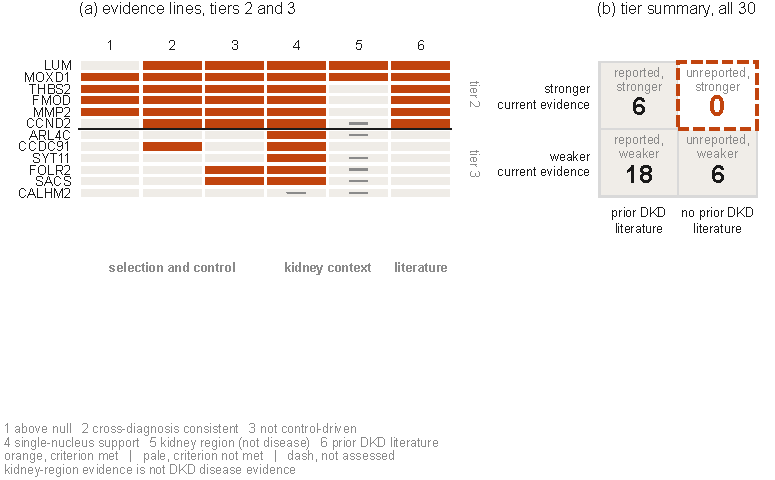
\includegraphics[width=\textwidth]{Fig10}
\caption{\textbf{Candidate evidence ledger.} \textbf{a} The 12 tier-2 and tier-3 candidates, which have either stronger current evidence or no prior DKD literature. The columns separate selection and control tests, human-kidney context, and literature status. Orange indicates a criterion met, pale a criterion not met, and a dash an assessment unavailable for that candidate; missing single-nucleus or regional-protein measurements are not scored as failures. The regional-protein column is the KPMP glomerulus-versus-tubulointerstitium contrast, which locates a protein rather than relating it to disease; it is not the diabetic-versus-non-diabetic protein evidence of Section~\ref{sec:proteome}, reported separately. The 18 tier-4 candidates are omitted here for legibility; Additional file~5 extends the matrix to all 30. \textbf{b} All 30 candidates classified by current evidence strength and prior DKD literature. The stronger-evidence/no-prior-literature cell is empty under the criteria fixed before the evidence was read.}\label{fig:candidates}
\smallskip\noindent{\footnotesize Alt text: Two panels. Left, a matrix of 12 candidate genes (rows) against evidence criteria (columns) grouped as selection and control tests, human-kidney context and literature status; orange cells are criteria met, pale cells criteria not met, dashes unavailable assessments. Right, all 30 candidates placed on a grid of current evidence strength against prior diabetic kidney disease literature, showing that no candidate is both strong and novel.}
\end{figure}


We report no novel biomarker. The corrected pipeline declining to promote its own uncorrected
output is the intended behaviour.

\subsection{Protein-level corroboration in two patient-independent datasets}\label{sec:proteome}

The candidate list is transcriptomic. Whether any of it survives a change of molecule is a
different question, and one the confounder analysis cannot answer. Two public cohorts measure
protein abundance in human kidney tissue under a diabetic-versus-non-diabetic contrast, in
patients unrelated to each other and to any cohort used here. Their control arms are not the
same: one enrolled healthy participants, the other non-diabetic pathology cases (Additional
file~6 records what each source states and what it leaves unstated). A SOMAscan aptamer panel of cortex
biopsies (23 diabetic kidney disease, 10 healthy; Mendeley 83k89shdx5 \cite{hirohama2023}) carries
841 of our
9,900 genes and 7 of the 30 candidates. Mass spectrometry of archival formalin-fixed cortex
(5 diabetic, 7 non-diabetic; PRIDE PXD041884 \cite{schwab2024}) quantifies 1,142 and 7. The two overlap in only
two candidates, so together they measure 12 of the 30.

The second cohort matters for a reason beyond sample size. Both of its arms are archival explant
cases from one institution, so the biopsy-versus-nephrectomy contrast that dominates the
transcriptome cohorts (Section~\ref{sec:procurement}) is absent from its design. That is a
weaker statement than procurement being matched: neither source reports ischaemia, fixation or
storage time, so pre-analytical exposure is unmeasured in both, exactly as it is in the
transcriptome cohorts.

Of the 12 candidates measured, 5 reach $q < 0.05$ in at least one cohort: \textit{MMP2},
\textit{MMP7}, \textit{THBS2} and \textit{CA10} on the aptamer panel, \textit{MMP7} and \textit{ACTN1} by
mass spectrometry (Table~\ref{tab:proteome}). Only \textit{MMP7} is significant in both, and only
there does the direction match the transcriptome in two measurement principles at once. The
other four rest on a single cohort each and should be read as such.

\begin{table}[h]
\caption{Candidates measured at the protein level in two patient-independent datasets. Neither shares patients with the other or with any transcriptome cohort used here, and the two use different measurement principles. Transcriptome effect is the mean across the harmonised cohorts; protein effect and $q$ are from the proteomic cohort named in each block.}\label{tab:proteome}
\begin{tabular}{@{}lrrrl@{}}
\toprule
Gene & Transcriptome $g$ & Protein $g$ & Protein $q$ & Direction \\
\midrule
\multicolumn{5}{@{}l}{\textit{SOMAscan aptamer panel; 23 DKD, 10 healthy (Mendeley 83k89shdx5)}} \\
\midrule
MMP2 & +1.58 & +1.71 & 0.008 & agrees \\
MMP7 & +1.82 & +2.04 & 0.008 & agrees \\
THBS2 & +1.78 & +1.31 & 0.013 & agrees \\
CA10 & -1.85 & -1.05 & 0.046 & agrees \\
LUM & +1.72 & +1.00 & 0.057 & agrees \\
TNFRSF12A & +0.95 & +0.32 & 0.587 & agrees \\
TNNT2 & -1.68 & +0.19 & 0.952 & differs \\
\midrule
\multicolumn{5}{@{}l}{\textit{LC-MS/MS of FFPE cortex; 5 DKD, 7 non-diabetic (PRIDE PXD041884)}} \\
\midrule
MMP7 & +1.82 & +3.34 & 0.045 & agrees \\
ACTN1 & +1.81 & +1.78 & 0.046 & agrees \\
CTNNBIP1 & -1.42 & +0.75 & 0.391 & differs \\
RNASE6 & +1.71 & -0.59 & 0.542 & differs \\
LUM & +1.72 & +0.43 & 0.587 & agrees \\
VCAN & +1.66 & +0.42 & 0.589 & agrees \\
COL1A2 & +2.01 & +0.39 & 0.614 & agrees \\
\botrule
\end{tabular}
\footnotetext{Neither cohort is genome-wide. The aptamer panel carries 841 of the 9,900 genes in the frozen space and 7 of the 30 candidates; the mass-spectrometry cohort quantifies 1,142 and 7. Twelve distinct candidates are measured in total, two (\textit{LUM}, \textit{MMP7}) in both. Absence means the protein was not measured, not that it failed. Pooled across the two cohorts, candidates reach $q<0.05$ more often than the proteins that are measured but not candidates (Cochran--Mantel--Haenszel $p = 0.030$; permutation without replacement $p = 0.035$; permutation with the background matched on abundance and peptide count $p = 0.039$).}
\end{table}

Two qualifications belong here. The first is about \textit{MMP7}: it is the headline finding
of the publication that produced the aptamer cohort \cite{hirohama2023}, so recovering it there
is not an independent observation: it is the same data reaching the same conclusion. What is
independent is the mass-spectrometry cohort, where the same protein moves the same way in
different patients on a different instrument.

The second is about what the mass spectrometer actually measured. Peptides are assigned to
proteins, and some peptides belong to more than one, so a quantified value is not automatically
specific to the gene it is labelled with. Of the 25 distinct peptides behind \textit{ACTN1},
only 8 are unique to it; the remaining 17 are shared with \textit{ACTN4}, \textit{ACTN2} and
\textit{ACTN3}, and \textit{ACTN4} is itself a podocyte gene, so that signal cannot be attributed to
\textit{ACTN1} alone. \textit{MMP7} carries an unambiguous accession but rests on 2 distinct
peptides. Additional file~6 reports aptamer identifiers, accessions and peptide counts for
every candidate in the table.

Neither cohort is significant on its own (Fisher $p = 0.11$ and $p = 0.18$): seven candidates
cannot separate a real enrichment from chance. Because their background rates differ widely
(28\% of measured non-candidates reach $q < 0.05$ on the panel, 11\% by mass spectrometry), they
must be pooled within strata rather than concatenated. Stratified, candidates reach $q < 0.05$
more often than the proteins measured alongside them: over the 14 candidate measurement
events, the Mantel--Haenszel common odds ratio against the stratum-specific backgrounds
is 3.3 (95\% CI 1.1--10.2), an interval wide enough that the size of the effect is not
established even though it excludes 1 (Cochran--Mantel--Haenszel \cite{mantel1959} $p = 0.030$;
permutation over 200,000 draws without replacement within each stratum $p = 0.035$,
against a null expectation of 2.7 significant candidates rather than the six observed). A
candidate set could reach that simply by being made of abundant, readily detected proteins, so
the permutation was repeated drawing each null protein from the background matched to that
candidate on abundance rank and, for the mass-spectrometry cohort, on peptide count: $p = 0.039$
(Additional file~6 reports the achieved balance). Direction agreement alone does not separate them
($p = 0.19$), which is expected: 60--67\% of background proteins already agree in direction.

The analysis plan (candidate versus measured non-candidate, Benjamini--Hochberg \cite{benjamini1995} $q < 0.05$,
direction as a separate test) was fixed on the first cohort and applied unchanged to the
second, which was located by a systematic search of PRIDE rather than chosen for its result.
Both cohorts are reported in full, including the two non-significant single-cohort tests and
the null direction test.

None of the five is novel. \textit{MMP2} and \textit{THBS2} are tier 2; \textit{MMP7}, \textit{CA10} and
\textit{ACTN1} tier 4. \textit{MOXD1}, the tier-2 candidate with the thinnest diabetic kidney disease
literature (1 paper, none proposing it as a marker, against 2 to 147 papers for the other
five in that tier), is on neither dataset. KPMP does quantify it in kidney tissue by mass
spectrometry, so it is measurable; it is simply not measured anywhere the contrast is
diabetic versus non-diabetic. The layer that could have promoted it does not do so.

%%=============================================================%%

\section{Discussion}\label{sec:discussion}
%%=============================================================%%

One boundary should be stated before anything else in this section. What follows is a warning
about cross-cohort omics benchmarking in general, but the quantification behind it is
concentrated in one disease, five discovery cohorts, with the two mechanisms then tested against
written predictions in two further tissues (Section~\ref{sec:xtissue}). That test turned both
from kidney observations into conditional statements. Verdict instability recurred in liver but
not in colon, whose cohorts agree about gene-wise effects far more than kidney or liver cohorts
do; the procurement confounder appeared wherever procurement was asymmetric and was prominent among
the most reproducible genes only where the asymmetry was shared by every cohort. The connectivity blind
spot does not depend on the disease either, as the simulation in Section~\ref{sec:modulesize}
shows. The magnitudes do. A reader should take the numbers below as measurements in three
tissues, and the two conditions, low effect concordance and a design shared across cohorts, as
hypotheses testable by the same procedure wherever more than two cohorts exist.

Cross-cohort consistency is a proxy for validity only when the cohorts differ in the ways that
matter. In public DKD transcriptomics they do not: every discovery contrast compares biopsies against
surgical or donor tissue, so the strongest shared signal is one associated with procurement, a dependence on reference tissue source that has since been observed independently in single-cell data \cite{menon2026}. This is a batch
effect in the sense of Leek et al.\ \cite{leek2010}, with the aggravating feature that it is
confounded with the outcome by design rather than merely correlated with it. Any criterion that
rewards consistency will find it, and no amount of additional cohorts of the same design will
reveal the problem: more cohorts make the confounder look more reproducible, not less.

The instability of benchmark verdicts has a simpler cause and a broader reach. With five cohorts
there are ten three-cohort configurations, and the sign of the reproducibility comparison differs
between them. That benchmark rankings shift with benchmark composition is not itself a new
observation \cite{boulesteix2013,jelizarow2010,ullmann2023,weber2019,norel2011}; what these
data add is the
magnitude in a setting where the practice of reporting a single configuration is universal, and
the observation that the two metrics behave differently: reproducibility flips sign, while the
mean external AUROC advantage does not. The cross-tissue test adds an association. The flips went
with cohorts that disagree about the disease signal: in colon, at a median effect correlation of
0.66, reversals were rare and small even after subsampling to kidney cohort sizes (two of five
replicates, at most 0.013). Three tissues cannot establish this as a necessary condition. Cross-cohort comparisons of reproducibility should be treated as descriptions of
a particular cohort collection rather than of the methods.

Practically, three things follow. Report reproducibility and validity as separate axes, since
they came apart measurably here. Include a confounder-matched contrast in the design: the 310
non-diabetic CKD biopsies in ERCB did more work than any algorithm in this study, and only two
of the public resources we used, ERCB and KPMP, contain such a comparator. And report pre-analytical variables (warm and
cold ischaemia time, fixation, and storage) in the SPREC \cite{betsou2010,lehmann2012} or
BRISQ \cite{moore2011} format. No DKD cohort we examined reports ischaemia time, which is why the
attribution in Section~\ref{sec:procurement} has to remain an inference; had these variables been
recorded, the confounder would be a covariate rather than a conjecture.

The handling score has an incidental use as a quality-control metric. It is computable per sample
from expression alone, requires no labels, and in these data tracks procurement route closely
enough to flag heterogeneous batches.

The cross-tissue test qualifies that use and the correction built on it. The module responds to
active inflammation as well as to handling: in colon, where both arms are endoscopic biopsies,
it rose in inflamed cases in 9 of 10 cohorts. As a quality-control flag it is interpretable only
alongside an inflammation score, and residualising on it in an inflamed tissue would remove
disease biology together with the artefact. In kidney that risk is bounded, since adjusting for
inflammation made the biopsy-versus-surgical effect larger rather than smaller. It is
nonetheless why we regard the score-based correction as tissue-conditional, and a control
obtained by the same procedure as the design alternative to prefer where clinically defensible and available.

\subsection{Limitations}\label{sec:limitations}

The empirical comparisons cover a limited set of established selection strategies,
including a custom co-expression hub comparator, rather than an exhaustive benchmark of
contemporary methods. The reversals recur under seven classical inner selectors and when the custom comparator is
replaced by the WGCNA package (Table~\ref{tab:selectors}), so they are not an artefact of the
reimplementation; the exclusion of the immediate-early module, by contrast, held for the
reimplementation and its 32 variants but not for the package on every fold, and appears to depend
on module detection rather than to be a property of connectivity criteria as a class. The magnitudes
reported apply to the implementations and cohort configurations examined here and should not be
generalised to entire method families. The audit procedure can be applied to additional selectors, but their sensitivity
to cohort composition remains to be evaluated.

The confounder-matched evidence rests on ERCB and KPMP; no other public DKD resource provides
non-diabetic kidney disease biopsies procured identically to the cases, so the specificity
argument rests on two resources. A partial external check is available and reported in
Section~\ref{sec:external}. The gate's background pass rate (8.3\%) and its permutation-based false-discovery estimate (16.7\%) are different quantities, as the footnote to Table~\ref{tab:corrections} sets out.

GSE104948 contributed both to discovery and to the matched-control specificity gate, so that gate is not a fully independent validation. Re-deriving the candidates with GSE104948 removed from discovery changes which genes are returned: 17 of the 30 survive, among them \textit{FMOD}, \textit{LUM}, \textit{MMP7} and \textit{MOXD1}. It does not change the conclusions drawn from the gate. The rate at which ranked genes clear the gate is no lower once the gate no longer shares a cohort with discovery (pipeline stage \texttt{sens\_no\_ercb\_check}), and the external replication holds (candidate median $|g_{\text{DKD}}| - |g_{\text{NSC}}|$ of $+1.00$ against $+1.02$, Mann--Whitney $p = 4.8 \times 10^{-16}$ against $5.1 \times 10^{-18}$). The overlap is real and partial; it is not what produces the specificity result.

The procurement effect did not replicate in heart, where explanted and donor hearts are handled similarly, but did appear in liver cohorts with biopsy cases and surgical or donor controls. Our simulation model is deliberately simple and does not capture
platform effects or realistic correlation structure beyond block correlation. The five discovery
cohorts remain few for LODO-based claims; the cohort-sensitivity analysis quantifies rather than
removes that limitation.

The cross-tissue test has limits of its own. Only three liver cohorts had asymmetric procurement,
one of them with a mixed case arm, and the liver core gene space retained 11 of the 19 module
genes. Procurement outside kidney was coded from series text and source publications, not from
recorded sample handling. Two predictions failed as written, and the explanations offered for
the failures, inflammation and effect concordance, were examined only post hoc and in three
tissues, too few to establish concordance as the condition for instability rather than one
correlate of it. The liver control substitution rests on 12 and 16 controls and is unresolved.

The central design claim rests on single-modality transcriptomics; the cross-modal and germline analyses support or bound it and are not its basis. Three things the phrase multi-omics can mean are supported to different degrees by public data, and only one is claimed here. Linking layers measured in the same participant could not be constructed from the public resources analysed. Cross-modal corroboration, which checks a candidate list in another layer in unmatched patients under a similar rather than identical comparison, is what Section~\ref{sec:proteome} does, against healthy participants in one cohort and non-diabetic pathology cases in the other. Within-layer discovery in the protein layer is not attempted, and Additional file~6 shows why it cannot yet be.

The obstacle to the first is worth stating precisely, because it is not that measurements are never paired. Of the 80 KPMP single-nucleus donors, the 27 in the operational DKD-proxy subset of Section~\ref{sec:cohorts} include 3 who also carry regional proteomics and 7 who carry spatial metabolomics. What is missing differs by layer. For regional proteomics it is the control arm: no participant in any control category carries it (0 of 12 healthy reference), so the contrast cannot be formed however many cases are paired. For spatial metabolomics both arms exist, 7 proxy and 6 healthy reference participants alongside transcriptomics, and the obstacle is the released format: imaging mass spectrometry distributed as image data rather than a per-participant matrix, behind a public API that exposes file counts without a retrieval path. No public resource therefore carries a multi-layer design complete enough to form a diabetic-versus-control contrast, and counting enrolment categories rather than recorded histories would have reached that conclusion for the wrong reason.

%%=============================================================%%

\section{Potential implications}\label{sec:conclusions}
%%=============================================================%%

A cross-cohort reproducibility comparison in omics biomarker discovery is a statement about a
particular collection of cohorts, not about the methods compared, unless it is accompanied by a
cohort-composition sensitivity analysis. In diabetic kidney disease the reproducibility verdict
changes sign across legitimate subsets of the same five cohorts, while the predictive verdict
does not, so the two should be reported as separate axes rather than as interchangeable summaries
of robustness. In a test against predictions fixed in advance, the same instability recurred in
liver but not in colon, whose cohorts agree closely about effects, so cross-cohort effect
concordance, computable before any method is run, indicates when a single configuration is least
trustworthy.

The signal that survives such a comparison most reliably in this disease is associated with
tissue procurement rather than with disease, because every discovery contrast compares biopsies with
surgical tissue. That is not a peculiarity of diabetic kidney disease: substituting a matched
comparator for the non-biopsy control removes most of the signal in all seven ERCB biopsy
diagnoses we could test, and diabetic nephropathy is unremarkable among them. The same module was
lower in biopsy cases than in surgical controls in liver, and was prominent among the most
reproducible genes only in kidney, where every cohort shares the asymmetry (8.0 genes against
0.6 in liver and 0.0 in colon). Whether a given method filters that confounder depends on the size of the block
it forms, not on the method's robustness. Residualisation on a specified control set and
surrogate-variable adjustment both remove most of it, at no significant cost in predictive
performance for the selector benchmarked here and at a cost that varies from none to about 0.1 AUROC across seven selectors, whereas correcting for batch by cohort cannot, because the confounder lies within
cohorts rather than between them. Because the module also rises with inflammation, correcting on
it is tissue-conditional, and a control obtained by the same procedure should be preferred
where clinically defensible and available.

What the correction buys is worth stating plainly, because it is not what a reader might expect.
It changes which genes are reported, not whether a biomarker can be reported at all. Only 14 of
the 30 candidates are the same genes before and after, and the corrected list moves towards
established biology, recovering 20 rather than 13 genes already proposed as diabetic kidney
disease markers. What it does not do is produce a defensible novel candidate: the cell requiring
a gene to be both strong in the data and absent from the literature is empty in both lists. The
value of removing this confounder is therefore diagnostic rather than generative. It tells a
reader that a list assembled without the correction is substantially a different list, and that
the difference does not run in the direction of novelty, which is the more useful thing to know
before any candidate set is carried forward.

We therefore recommend that studies of this kind report a cohort-composition interval alongside
any reproducibility claim, include a confounder-matched contrast in the design, and report
pre-analytical variables to the SPREC or BRISQ standard, which would convert the confounder
described here from an inference into a measurable covariate.

%%=============================================================%%

\section{Methods}\label{sec:methods}
%%=============================================================%%

The study has two layers. The first layer is a conventional
cross-cohort benchmark: retrieve public cohorts, audit them for patient reuse, harmonise them
into one frozen gene space, and compare four selection strategies under leave-one-dataset-out
evaluation. The second layer is the set of controls placed around that benchmark, namely the
random-signature and permuted-label nulls, the sweep over cohort subsets, the procurement
contrast, and the substitution of the control group. Cohort assembly and harmonisation are described under Data description (Sections~\ref{sec:cohorts} and~\ref{sec:harmonisation}); Section~\ref{sec:selectors}
the four strategies, Section~\ref{sec:nulls} the nulls and the sensitivity sweeps,
Section~\ref{sec:corrections} the confounder score and the corrections benchmarked against it,
Section~\ref{sec:xtmethods} the test of both mechanisms in liver and colon,
and Section~\ref{sec:implementation} how each reported number is regenerated from source data.


\subsection{Selection methods}\label{sec:selectors}

Four strategies were compared, all on the same gene space and the same folds.

\textbf{DEG\_meta.} Per-cohort Welch $t$-statistic combined across cohorts by Stouffer's method
weighted by $\sqrt{n}$ \cite{whitlock2005}. The plain effect-size approach.

\textbf{WGCNA\_hub.} Soft-thresholded correlation network, module defined by gene--trait
correlation, genes ranked by intramodular connectivity: a connectivity-based hub ranking in the
manner of WGCNA \cite{langfelder2008}, of the kind used by prior DKD work \cite{feng2021}. It is
implemented directly rather than called from the reference package, and it departs from the
canonical pipeline in three respects: the soft power is fixed at $\beta = 6$ rather than chosen
by the scale-free topology criterion, modules are defined by gene--trait correlation rather than
by dynamic tree cut on the topological overlap matrix, and hubs are ranked by intramodular
connectivity rather than by module membership. We do not claim this reproduces WGCNA. Table~\ref{tab:comparator} states element by element what is shared and what is not; Additional file~1 rebuilds the comparator across those axes and shows that the ranking behaviour Section~\ref{sec:modulesize} rests on is unchanged in every variant.

\begin{table}[h]
\caption{What the correlation-module comparator shares with the canonical WGCNA pipeline, and where it departs. Additional file~1 tests whether any departure changes a conclusion.}\label{tab:comparator}
\footnotesize
\setlength{\tabcolsep}{4pt}
\begin{tabular}{@{}p{24mm}p{41mm}p{41mm}p{15mm}@{}}
\toprule
Element & Canonical WGCNA & Used here & Status \\
\midrule
Similarity measure & Pearson correlation & Pearson correlation & same \\
Adjacency & signed or unsigned power & unsigned power & restricted \\
Soft-threshold power & chosen by scale-free fit & fixed at $\beta = 6$ & differs \\
Module detection & TOM distance, dynamic tree cut & clustering on correlation distance & differs \\
Hub score & kME, eigengene correlation & intramodular connectivity kIN & differs \\
Module eigengene & first principal component & not computed & absent \\
\botrule
\end{tabular}
\footnotetext{The departures are why the manuscript calls this a correlation-module comparator rather than WGCNA. We do not claim it reproduces the reference package; the package itself was also run as a second comparator (Section~\ref{sec:sensitivity}).}
\end{table}

\textbf{RBS.} Cross-cohort stability selection (robust biomarker score), used here as an instrument rather than
proposed as a contribution: it stands in for the family of stability-selection approaches
\cite{meinshausen2010} so that the benchmark contains a representative of that family, and no
claim of novelty attaches to it. Bootstrap selection is run inside each cohort separately and
aggregated across cohorts, never on the pooled matrix. In the headline benchmark the inner selector is ReliefF, run on $B = 200$ class-stratified bootstrap replicates per cohort at $K = 50$. Let $\pi_{cj}$ be the fraction of those replicates of cohort $c$ in which gene $j$ is selected. The four components are importance $I_j$, the selector score of gene $j$ divided by the largest score in the same replicate, averaged over replicates and cohorts, so that a gene the selector never touches scores zero; stability $S_j = M^{-1} \sum_c \pi_{cj}$; cross-cohort reproducibility $R_j$; and perturbation robustness $P_j$, the selection frequency of gene $j$ over 40 refits per cohort under class-stratified 70\% subsampling, Gaussian noise at half the gene-wise standard deviation, masking of 20\% of genes, and a synthetic batch shift, computed only for the 300 genes ranked highest by $I_j S_j R_j$ so that perturbation stress-tests candidates rather than discovers them:

\begin{equation}
R_j = \delta_j \exp\Bigl( \frac{1}{M} \sum_{c} \log (\pi_{cj} + \epsilon) \Bigr) , \qquad
\mathrm{RBS}_j = \delta_j \exp\Bigl( \frac{\sum_k w_k \log (V_{kj} + \epsilon)}{\sum_k w_k} \Bigr) ,
\label{eq:rbs}
\end{equation}

where $V_{\cdot j} = (I_j, S_j, R_j, P_j)$, $w = (1, 1, 2, 1)$, $\epsilon = 10^{-3}$ inside $R_j$ and $10^{-6}$ in the combination, and $\delta_j \in \{0, 1\}$ is the
sign-concordance gate, equal to $1$ only when $g_{cj}$ carries the same non-zero sign in every
cohort. The geometric mean requires a gene to be adequate on all four components rather
than to buy its way in on one, and the gate is hard rather than a soft penalty. Baseline selectors within the bootstrap were compared (univariate
$F$, LASSO \cite{tibshirani1996}, elastic net \cite{zou2005}, mRMR \cite{peng2005}, ReliefF \cite{kononenko1994}, random forest \cite{breiman2001}, Boruta \cite{kursa2010}), all implemented directly rather
than through packages that pin older \texttt{numpy}/\texttt{scikit-learn} versions.

\textbf{RBS\_orth.} RBS after residualising every gene on a per-sample handling score
(Section~\ref{sec:corrections}).

Two cohort sets are used and the distinction matters when reading the tables below. The headline
benchmark and its nulls run on the four cohorts fixed before the analysis began (GSE30528,
GSE96804, GSE104948, GSE142025). The cohort-composition sweep of Section~\ref{sec:sensitivity}
adds GSE294519 as a fifth, because that analysis exists precisely to vary the cohort set and
a wider set of compositions makes it stronger.

Evaluation is leave-one-dataset-out (LODO). Write the harmonised cohorts as $D_1,\dots,D_M$. For held-out cohort $m$ the training set is $T_m = \bigcup_{j \neq m} D_j$; a selection strategy $S$ returns the top-$K$ gene set $G_m^{(K)} = S(T_m,K)$; a plain $L_2$ logistic model $f_m$ is fitted on $T_m$ restricted to those genes and assigns each sample $i \in D_m$ a score $s_i = f_m(x_i)$. The classifier is deliberately simple because the object of study is the features, not the classifier.

Let $P_m$ and $N_m$ be the case and control samples of $D_m$, with $n_1 = |P_m|$ and $n_0 = |N_m|$. External AUROC is the Mann--Whitney statistic, ties counted as half:
\begin{equation}
\mathrm{AUROC}_m = \frac{1}{n_1 n_0}
\sum_{i \in P_m} \sum_{j \in N_m}
\Bigl[ \mathbf{1}(s_i > s_j) + \tfrac{1}{2}\mathbf{1}(s_i = s_j) \Bigr] ,
\label{eq:auroc}
\end{equation}
and the reported value is the mean over folds, $\overline{\mathrm{AUROC}} = M^{-1}\sum_{m=1}^{M} \mathrm{AUROC}_m$. The tie term matters here because several cohorts are small enough for scores to tie exactly.

The second axis is reproducibility, the agreement between the gene sets selected on different training sets:
\begin{equation}
J = \binom{M}{2}^{-1} \sum_{m < m'}
\frac{|G_m^{(K)} \cap G_{m'}^{(K)}|}{|G_m^{(K)} \cup G_{m'}^{(K)}|} .
\label{eq:jaccard}
\end{equation}
The two axes are reported separately throughout and are not interchangeable: Section~\ref{sec:sensitivity} shows they disagree.

\textbf{Effect size.} Every effect size reported here is Hedges' $g$ \cite{hedges1981}, the standardised
mean difference with the small-sample correction. For gene $j$ with case and control
groups of size $n_1$ and $n_0$,

\begin{equation}
g_j = \frac{\bar{x}_{1j} - \bar{x}_{0j}}{s_{p,j}} \Bigl( 1 - \frac{3}{4(n_1 + n_0) - 9} \Bigr) , \qquad
s_{p,j}^{2} = \frac{(n_1 - 1) s_{1j}^{2} + (n_0 - 1) s_{0j}^{2}}{n_1 + n_0 - 2} .
\label{eq:hedges}
\end{equation}

The specificity gate keeps genes with $|g_j| \ge 0.5$ in the diabetic-versus-other-
kidney-disease contrast, averaged over the two ERCB compartments.

\subsection{Null controls and uncertainty}\label{sec:nulls}

Two nulls are computed per fold and per signature size. For the random-signature null, $B = 300$ gene sets $R_1,\dots,R_B$ of the same size $K$ are drawn uniformly from the same frozen gene space, and the model is refitted and rescored on the same fold with real labels. An observed AUROC is reported as its position in that null,
\begin{equation}
\pi_m = \frac{1}{B} \sum_{b=1}^{B}
\mathbf{1}\bigl( \mathrm{AUROC}_m^{(R_b)} < \mathrm{AUROC}_m \bigr) ,
\label{eq:percentile}
\end{equation}
never as the raw value. The second null permutes the case/control labels within each cohort and leaves everything else unchanged, so it measures what the evaluation returns when no signal exists at all. This control follows Venet et al.\ \cite{venet2011}, who showed that most random signatures are significantly associated with outcome in breast cancer.

All method comparisons use a paired patient-level bootstrap of $R = 40$ replicates, stratified by cohort and class, with the entire LODO evaluation, selection included, re-run inside each replicate. The interval is formed on the paired difference computed within a replicate,
\begin{equation}
\Delta^{(r)} = \overline{\mathrm{AUROC}}_{A}^{(r)}
- \overline{\mathrm{AUROC}}_{B}^{(r)} ,
\qquad r = 1,\dots,R ,
\label{eq:paired}
\end{equation}
and quoted as the 2.5th and 97.5th percentiles of $\Delta^{(1)},\dots,\Delta^{(R)}$. Pairing within the replicate is what makes the interval informative: the two methods see identical patients, so the cohort-to-cohort variance that dominates the marginal AUROC cancels. Resampling folds (3--5 units) or the pairwise
Jaccard values (which are correlated) does not support an interval. $R$ is small for a percentile interval because each replicate repeats the whole evaluation, selection included; it is set by compute, and the intervals should be read as bootstrap ranges whose finest resolvable two-sided $p$ is $2/R = 0.05$.

Cohort-composition sensitivity is assessed exhaustively: every subset of the five discovery
cohorts of size 2--5 (26 subsets) receives a complete benchmark, with 30 inner bootstrap replicates per cohort rather than the 200 of the headline run, since the sweep asks which method wins rather than for its score to the third decimal.

\subsection{Confounder score, corrections and simulation}\label{sec:corrections}

The immediate-early gene (IEG) module (\textit{FOS}, \textit{FOSB}, \textit{JUN}, \textit{JUNB},
\textit{EGR1}, \textit{ATF3}, \textit{DUSP1}, \textit{ZFP36}, \textit{NR4A1}, \textit{NR4A2},
\textit{BTG2}, \textit{EGR2}, \textit{EGR3}, \textit{IER2}, \textit{KLF2}, \textit{KLF4},
\textit{SOCS3}, \textit{DUSP2}, \textit{JUND}) is a per-sample, label-free proxy for tissue
handling; its mean $z$-score over that module is the handling score $h_i$ of sample $i$.

Residualisation removes that axis from every gene. The slope is estimated \emph{within} class,
not over all samples: because cases are biopsies and controls are not, $h$ is nearly collinear
with case status, and a total slope would absorb the disease difference itself. Writing $\tilde{h}$
and $\tilde{x}_j$ for $h$ and gene $j$ centred inside each class,

\begin{equation}
\beta_j = \frac{\tilde{h}^{\top} \tilde{x}_j}{\tilde{h}^{\top} \tilde{h}} , \qquad
x_{ij}^{\text{corr}} = x_{ij} - \lambda (h_i - \bar{h}) \beta_j ,
\label{eq:resid}
\end{equation}

with $\lambda = 1$ for full removal. Corrections compared: no correction; residualisation on
the handling score by Eq.~(\ref{eq:resid}); RUVg with the module as negative controls; RUVg with
empirically chosen controls (the least associated genes) \cite{risso2014}; a surrogate-variable
adjustment protecting the design \cite{leek2007}; and ComBat with cohort as batch
\cite{johnson2007}.

The simulation uses a generative model with a disease block and a confounder block, each
with within-block correlation, cohort-specific effect heterogeneity ($\sigma_d$, $\sigma_c$ drawn once per cohort),
and a confounder correlated with case status by $\rho$. Block sizes, $\rho$, heterogeneity and
cohort count are swept. The stability arm was run both with a simplified stand-in and with the
actual RBS implementation; conclusions were identical.

\subsection{Predictions fixed before the liver and colon data were read}\label{sec:xtmethods}

The two findings make different predictions outside kidney. Instability of reproducibility
verdicts under a change of cohorts is a statistical claim and should appear in any tissue; a
procurement confounder should become reproducible only where every cohort shares the same
asymmetry between arms. Two tissues separate these. In liver with metabolic
dysfunction-associated steatohepatitis (MASH), procurement is asymmetric in some cohorts (needle
biopsy cases, living-donor or surgical controls) and matched in others (both arms needle
biopsies, or both intraoperative at bariatric surgery); in ulcerative colitis (UC), both arms
are endoscopic biopsies in every cohort. Three predictions (Section~\ref{sec:xtissue}) were
written after reading only series- and sample-level metadata and before any expression value was
downloaded, and the file's SHA-256 digest and time stamp were recorded when it was written. A
second file stating post hoc analyses was written and hashed after the verdicts were known and
before those analyses ran. A pipeline stage verifies both digests on every run, and both files
are reproduced in Additional file~7. The digests are local records: they establish that neither
file changed after it was written, not an externally certified date, since no third-party registry
entry exists. We therefore call these predictions stated and hash-fixed before the analysis.

Cases were MASH against histologically normal liver and actively inflamed UC colon against
normal control colon, one sample per subject, with ileal and Crohn's disease samples excluded.
Procurement was coded per arm from the series text, the sample fields and the source
publication, with its evidence recorded, before any effect was computed. In each tissue five
core cohorts, matching the five kidney discovery cohorts, entered the composition sweep; the
remaining eligible cohorts entered only the per-cohort module test (Additional file~7). Patient
reuse across series from the same group or platform was audited on the expression values
themselves: a sample whose best-correlated partner in another series reached $r \ge 0.9999$ was
called identical, and a pair of series whose median gap between the best and second-best partner
correlation exceeded five times that of an unrelated same-platform pair was called re-processed
from shared individuals. The audit confirmed GSE59071 as a subset of GSE75214 (116 identical
samples) and GSE17470 as overlapping GSE24807 (9 identical), and both were excluded; it also
found GSE48452 and GSE61260 likely to share individuals (median gap 0.0109 against 0.0016), and
GSE61260, whose deposited matrix could not be mapped to samples, was not analysed.

Microarrays were mapped to Entrez identifiers through the platform annotation, RNA-seq counts
were transformed to $\log_2(\text{CPM}+1)$ after keeping genes with CPM $\ge 1$ in at least
20\% of samples, and probes were collapsed by maximum mean, as for kidney. Selection used the
genes shared by each tissue's five core cohorts: 7,805 in liver, including 11 of the 19
immediate-early genes, and 15,789 in colon, including all 19. The four strategies, $K = 50$, the
inner selector, the soft-thresholding power and the inner $B = 30$ of the kidney composition
sweep were reused by calling the same code, and the kidney reference was recomputed with it. The
per-cohort effect $g_{\text{IEG}}$ is Hedges' $g$ of the handling score, case minus control,
with a 95\% interval from 1,000 bootstrap resamples within arms and a percentile against 2,000
random gene modules of the same size.

Four post hoc analyses followed the plan. Control substitution was repeated in GSE48452, which
contains MASH cases with two control groups: liver from oncological surgery and histologically
normal liver from obese individuals at the same bariatric operations as most cases. The
immediate-early effect was adjusted for inflammation by regressing the standardised handling
score on case status within each cohort, with and without an inflammation score fixed in advance
from 13 genes sharing none with the module (\textit{PTPRC}, \textit{CD14}, \textit{CD68},
\textit{FCGR3A}, \textit{S100A8}, \textit{S100A9}, \textit{LCN2}, \textit{CXCL8}, \textit{IL1B},
\textit{TNF}, \textit{SAA1}, \textit{MMP3}, \textit{CHI3L1}). Cross-cohort effect concordance
was defined as the median pairwise Spearman correlation of gene-wise $g$ across the five core
cohorts, and colon was re-run with each core cohort subsampled without replacement to the case and
control counts of a kidney discovery cohort, in five replicates. Finally, the liver RNA-seq filter
was relaxed to a raw count of at least 1 in 20\% of samples to test whether the liver module
coverage affected the result.

\subsection{Implementation}\label{sec:implementation}

All analyses are implemented in Python 3.14 against \texttt{numpy}, \texttt{scipy},
\texttt{pandas}, \texttt{scikit-learn} and \texttt{matplotlib}, with pinned versions. The
pipeline runs from a single entry point covering 133 declared stages, of which 122 reproduce the
results reported here; every stage that resamples takes a fixed seed, and reruns reproduce the
reported numbers, with the run-time dependence on external reference resources recorded
under Regeneration below.

\textbf{Use of AI tools.} Claude Code (Anthropic) and ChatGPT (OpenAI) assisted with code
development and refactoring, proposals for control analyses, language editing and revision of
author-written text, and the code that draws the figures; no figure or result was generated by
an AI model directly. Numerical results were computed from the cited datasets or explicitly
described simulations using the analysis code. Automated checks were used to assess numerical
consistency and provenance. The authors reviewed the code, analyses and manuscript and take
responsibility for the final content.

Every comparator is implemented directly rather than called from a reference package, for
reasons of speed and single-environment reproducibility set out in Additional file~1. That file
also states, for each comparator, what it shares with its reference definition and where it
departs, and reports the variant grid establishing that no conclusion here depends on those
departures. Readers assessing the comparisons in Sections~\ref{sec:sensitivity}
and~\ref{sec:modulesize} should read it alongside them.

%%=============================================================%%

\section*{Availability of source code and requirements}
\begin{itemize}
  \item \textbf{Project name:} dkd-cross-cohort-audit
  \item \textbf{Project home page:} \url{https://github.com/kdh6126/dkd-cross-cohort-audit}
  \item \textbf{Operating system(s):} Platform independent (developed and run on Windows 11)
  \item \textbf{Programming language:} Python 3.14; R 4.6.1 for the reference WGCNA comparator only
  \item \textbf{Other requirements:} Python packages pinned in requirements.txt (numpy 2.5.2, scipy 1.18.1, pandas 3.0.5, scikit-learn 1.9.0, matplotlib 3.11.1, pyarrow 25.0.1, h5py 3.16.0); R package WGCNA 1.74; a LaTeX distribution to rebuild the manuscript
  \item \textbf{License:} MIT
  \item \textbf{Restrictions to use by non-academics:} None
  \item \textbf{Archived version:} \url{https://doi.org/10.5281/zenodo.23051697} (version 1.0.0)
\end{itemize}

\section*{Data availability}

The data sets supporting the results of this article are available in the Zenodo repository, \url{https://doi.org/10.5281/zenodo.23051697} \cite{kim2026zenodo}, with the primary public records listed below.

All data supporting the conclusions of this article are publicly available, and all code
required to regenerate every figure and table is openly released.

\textbf{Primary data.} All transcriptome cohorts analysed here are available from the Gene
Expression Omnibus (\url{https://www.ncbi.nlm.nih.gov/geo/}) under accessions GSE30528,
GSE30529, GSE96804, GSE104948, GSE104954, GSE142025, GSE294519, GSE162830, GSE175759,
GSE142153, GSE1009, GSE111154, GSE20602 and GSE5406. The three series excluded by the cohort
audit for patient-level reuse are GSE30122, GSE47183 and GSE99340. The liver cohorts of
Section~\ref{sec:xtissue} are GSE89632, GSE48452, GSE162694, GSE126848, GSE83452, GSE66676,
GSE63067 and GSE24807, and the colon cohorts GSE75214, GSE87466, GSE179285, GSE11223, GSE47908,
GSE38713, GSE53306, GSE16879, GSE48958 and GSE13367; GSE59071, GSE17470 and GSE61260 were
excluded by the reuse audit or for an unmappable matrix. Single-nucleus data are
available from the Kidney Precision Medicine Project Atlas (\url{https://atlas.kpmp.org/}).

\textbf{Other public resources.} The two protein datasets used for the orthogonal corroboration in
Section~\ref{sec:proteome} are the SOMAscan aptamer panel of kidney cortex biopsies
(Mendeley Data 83k89shdx5, \url{https://doi.org/10.17632/83k89shdx5.1}) and the FFPE cortex
LC-MS/MS dataset (PRIDE \url{https://www.ebi.ac.uk/pride/}, accession PXD041884). The
germline test uses the diabetic-kidney-disease genome-wide association study GCST90179152
from the GWAS Catalog (\url{https://www.ebi.ac.uk/gwas/}). The plasma metabolome used in
Sections~\ref{sec:auroc-null} and~\ref{sec:external} is study ST003255 of the Metabolomics
Workbench (\url{https://www.metabolomicsworkbench.org/}).

%% BEGIN AVAILABILITY
\textbf{Processed data.} The harmonised per-cohort expression matrices, the frozen 9,900-gene
Entrez space, the probe-to-gene mapping, and the sample-level phenotype tables including the
procurement annotation are deposited at \url{https://doi.org/10.5281/zenodo.23051697} under CC BY 4.0. The cohort audit is
distributed with them as a relational database whose views encode the exclusion and overlap
rules stated in Section~\ref{sec:cohorts}, so that the audit is enforced by the schema rather
than by prose.

\textbf{Code.} All analysis code is available at \url{https://github.com/kdh6126/dkd-cross-cohort-audit} under the MIT licence \cite{kim2026zenodo}, archived at \url{https://doi.org/10.5281/zenodo.23051697}.
%% END AVAILABILITY

\textbf{Regeneration.} The repository provides a single entry point, \texttt{run\_all.py},
covering 133 declared stages, of which 122 reproduce the results reported here. Running
\texttt{python run\_all.py -{}-paper} runs the 104 of them that the figures, tables and
reported numbers depend on. That set is a static list in the code, and before running anything
\texttt{-{}-paper} checks it against a dependency closure computed from the declared outputs of
every stage and the inputs its command line and source refer to; the run aborts if the two
diverge. Inputs are inferred statically, so the check constrains the set rather than proving it
complete.
Each stage declares the files it produces, so a run resumes where it stopped, and every stage
that resamples takes a fixed seed.

Reruns are not bit-identical, and we state why rather than round it away. Of the 104 stages,
12 query external resources at run time (PubMed, the KPMP Atlas, KEGG, Reactome and GEO),
so their outputs can depend on the state of the resource on the day of the run, although the
four cross-tissue stages among them download fixed GEO series. The reported
field observed to change was the PubMed novelty count: rerunning on 2026-09-02 moved one
gene from 22 to 23 papers. Tier assignments, which are what the manuscript reports, did not
change for any of the 30 candidates, and each candidate's query string, query date and returned
identifiers are recorded in Additional file~6 so that any later divergence is traceable.


\section*{Declarations}
\bmhead{List of abbreviations}
%%=============================================================%%

AUROC: area under the receiver operating characteristic curve; BRISQ: Biospecimen Reporting for
Improved Study Quality; CKD: chronic kidney disease; DKD: diabetic kidney disease; ERCB: European Renal cDNA Bank; GEO: Gene Expression Omnibus; IEG: immediate-early
gene; KPMP: Kidney Precision Medicine Project; LODO: leave-one-dataset-out; MASH: metabolic
dysfunction-associated steatohepatitis; RBS: robust biomarker
score; RUVg: remove unwanted variation using control genes; SPREC: Standard PREanalytical Code;
UC: ulcerative colitis; WGCNA: weighted gene co-expression network analysis.


%%=============================================================%%

\bmhead{Ethics approval and consent to participate}

Not applicable. This study analysed only previously published, de-identified human data obtained
from public repositories, and generated no new human or animal data.

\bmhead{Consent for publication}

Not applicable. The manuscript contains no data from any individual person.

\bmhead{Competing interests}

The authors declare that they have no competing interests.

\bmhead{Funding}

%% BEGIN FUNDING
This work was supported by the National Research Foundation of Korea (NRF) grant funded by the Korean government (MSIT) [grant number RS-2026-25524613]; an internal research grant of the Electronics and Telecommunications Research Institute (ETRI) [grant number 25YT1400]; and the Culture, Sports and Tourism R\&D Program through the Korea Creative Content Agency grant funded by the Ministry of Culture, Sports and Tourism in 2024 [grant number RS-2024-00398310]. The funders had no role in the design of the study, in the collection, analysis and interpretation of data, or in writing the manuscript.
%% END FUNDING

\bmhead{Authors' contributions}

%% BEGIN CONTRIBUTIONS
DK conceived the study, designed the methodology, implemented the analysis pipeline, curated and harmonised the data, performed the formal analysis, carried out the analyses, designed and ran the validation and control analyses, produced the figures, provided study resources, wrote the original draft and reviewed and edited the manuscript. MB, JP, HL and HJL designed the methodology, curated and harmonised the data and reviewed and edited the manuscript. SL acquired funding, administered the project, supervised the work and reviewed and edited the manuscript. All authors read and approved the final manuscript.
%% END CONTRIBUTIONS

\bmhead{Acknowledgements}

%% BEGIN ACKNOWLEDGEMENTS
The results reported here are in whole or in part based upon data generated by the Kidney Precision Medicine Project. Accessed August 24, 2026. \url{https://www.kpmp.org}. The KPMP study is supported by the National Institute of Diabetes and Digestive and Kidney Diseases (NIDDK). We acknowledge the essential contribution of the patient participants who consented to kidney biopsy for research.

We also thank the European Renal cDNA Bank consortium and the investigators who deposited the public datasets analysed here, without which this study would not have been possible.
%% END ACKNOWLEDGEMENTS

%%=============================================================%%
%% Figure legends. Figures are supplied as separate files.     %%
%%=============================================================%%


\bmhead{Disclosure of use of AI-assisted tools including generative AI}

Claude Code (Anthropic) and ChatGPT (OpenAI) assisted with code
development and refactoring, proposals for control analyses, language editing and revision of
author-written text, and the code that draws the figures; no figure or result was generated by
an AI model directly. Numerical results were computed from the cited datasets or explicitly
described simulations using the analysis code. Automated checks were used to assess numerical
consistency and provenance. The authors reviewed the code, analyses and manuscript and take
responsibility for the final content. The tools are cited as \cite{claudecode2026,chatgpt2026}.

\section*{Additional files}


\textbf{Additional file 1 (PDF).} Comparator implementation and its validation: what the WGCNA hub
ranking used here does and does not share with the canonical pipeline, the scale-free topology
fit across soft powers, the 32-variant grid testing whether
Section~\ref{sec:modulesize} depends on those choices, the provenance of the remaining
selectors, and the block-size simulation run with the RBS implementation.

\textbf{Additional file 2 (PDF).} Cohort audit report, including the patient-identifier evidence for
the three excluded series and the residual overlap that could not be removed.

\textbf{Additional file 3 (XLSX).} Per-cohort harmonisation summary and the complete candidate table
with every line of evidence.

\textbf{Additional file 4 (XLSX).} Per-diagnosis results underlying Section~\ref{sec:external}:
the effect vectors for each ERCB diagnosis under both control definitions, the three
external validation datasets, the KPMP single-nucleus contrast summary, and the KPMP modality
table by diagnosis.

\textbf{Additional file 5 (PDF).} Candidate evidence over all 30 specificity-gated candidates: Figure~\ref{fig:candidates} extended to include the 18 tier-4 candidates omitted from the main text for legibility.

\textbf{Additional file 6 (PDF).} The two proteomic cohorts used in Section~\ref{sec:proteome}:
what each source publication and repository record states about case and control definition,
tissue, procurement route and pre-analytical reporting, together with the abundance- and
peptide-count-matched permutation and its achieved balance, and a negative control asking
whether the two proteomic datasets could have produced a candidate list on their own.

\textbf{Additional file 7 (XLSX).} The test in liver and colon (Section~\ref{sec:xtissue}): the
registered predictions and post hoc plan with their SHA-256 digests; every cohort considered,
with platform, case and control definitions, procurement coding per arm with its evidence, and
inclusion status; the value-vector reuse audit; per-cohort immediate-early effects; the
composition sweeps; and the post hoc analyses.
%%=============================================================%%

\bibliographystyle{bib-vancouver}
\bibliography{dkd-references,giga-extra}
\end{document}